% Modified for use with IJQC - Madhusudan Singh Copyright (C) (2011). All rights reserved.
\documentclass[12pt]{article}

\setlength{\oddsidemargin}{0in}  %left margin position, reference is one inch
\setlength{\textwidth}{6.5in}    %width of text=8.5-1in-1in for margin
\setlength{\topmargin}{-0.5in}    %reference is at 1.5in, -.5in gives a start of about 1in from top
\setlength{\textheight}{9in}     %length of text=11in-1in-1in (top and bot. marg.) 


\usepackage{amsmath,amssymb}
\usepackage{graphicx}% Include figure files
\usepackage{color}% Include colors for document elements
\usepackage{dcolumn}% Align table columns on decimal point
\usepackage{bm}% bold math
\usepackage[authoryear, semicolon]{natbib}
\usepackage{amsfonts}
\usepackage[utf8]{inputenc}
\usepackage{url}
\usepackage{lineno}
\usepackage{endfloat}
\usepackage{subfigure}
\usepackage{microtype}
\usepackage{booktabs}
\DisableLigatures{encoding = *, family = * }


\title{\textbf{A Hierarchical Bayesian Analysis of Parasite Prevalence and Socio-Cultural Outcomes:} \\
The Role of Structural Racism and Sanitation Infrastructure  }

\author{Cody T Ross\thanks{Department of Anthropology, University of California, Davis, 95616}, Bruce Winterhalder$^*$
}
\begin{document}

\maketitle

\begin{small}
\begin{abstract}
\textbf{Objectives:} We conduct a revaluation of the Thornhill and Fincher research project on parasites using finely-resolved geographic data on parasite prevalence, individual-level socio-cultural data, and multi-level Bayesian modeling. In contrast to the evolutionary psychological mechanisms linking parasites to human behavior and cultural characteristics proposed by Thornhill and Fincher, we offer an alternative hypothesis that structural racism and differential access to sanitation systems drive both variation in parasite prevalence and differential behaviors and cultural characteristics.
 
\textbf{Methods:}	We adopt a Bayesian framework to estimate parasite prevalence rates in fifty-one districts in eight Latin American countries using the disease status of 170,220 individuals tested for infection with the intestinal roundworm \textit{Ascaris lumbricoides} \citep{Hurlimann2011}. We then use district-level estimates of parasite prevalence and individual-level social data from 5,558 individuals in the same fifty-one districts \citep{LB2008} to assess claims of causal associations between parasite prevalence and socio-cultural characteristics.
 
\textbf{Results:} We find, contrary to Thornhill and Fincher, that parasite prevalence is \textit{positively} associated with preferences for democracy, \textit{negatively} associated with preferences for collectivism, and \textit{not} associated with violent crime rates or gender inequality.  A positive association between parasite prevalence and religiosity, as in \citet{Fincher2012}, and a negative association between parasite prevalence and achieved education, as predicted by \citet{Eppig2010}, become negative and unreliable when reasonable controls are included in the model.  We find support for all predictions derived from our hypothesis linking structural racism to both parasite prevalence and cultural outcomes. 

\textbf{Conclusions: }We conclude that best practices in biocultural modeling require examining more than one hypothesis, retaining individual-level data and its associated variance whenever possible, and adopting multi-level techniques suited to the structuring of the data.  
 \end{abstract}
\end{small}


\clearpage
\linenumbers
\section{Introduction}
\subsection{Introduction}
	We estimate parasite prevalence in fifty-one districts in eight Latin American countries using the disease status of 170,220 individuals tested for infection with the intestinal roundworm \textit{Ascaris lumbricoides} \citep{Hurlimann2011}. Estimates of parasite prevalence are derived in a full Bayesian framework using district-level binomial probability densities, and a prior, estimated from the data, under two geographic levels of hierarchical partial pooling. We utilize district-level parasite prevalence estimates, and individual-level demographic and social data from 5,558 individuals in the same fifty-one districts \citep{LB2008}, to retest the hypotheses presented by \citet{Fincher2012}, \citet{Thornhill2011}, \citet{Eppig2010}, \citet{Thornhill2009}, and \citet{Fincher2008} (hereafter, TFE) in a joint probability model.  Finding results contrary to those presented in TFE, \citep[as have other researchers attempting to replicate their findings, see][]{hackman2013fast}, we argue that much of the structuring that they observe between parasite prevalence and cultural covarites (preferences for democracy, collectivism, women's rights, intelligence/education, violence, and religiosity) is due to neglected variable bias and spurious correlation.  Specifically, we demonstrate that proxy variables linked to structural racism, such as ethnicity and differential access to sanitation and sewage systems, can explain both the structured variation in parasite prevalence across districts, as well as the associated variation in social and cultural characteristics of individuals across districts.

\subsection{The Biology of Poverty}
Evolutionary anthropologists often look for adaptive explanations for cross-cultural or cross-population differences in cultural or behavioral outcomes \citep{bogin2007life}.  It is now widely recognized that such differences are not necessarily or even commonly indicative of genetic divergence, but more often represent socio-cultural responses to proximate environmental conditions.  Critical differences in cultural and biological outcomes often arise as a function of ethnicity and social inequality \citep{gravlee2009race}.  Nutrition, educational attainment, and socio-economic status are often associated with health status, and hence parasite prevalence, in many cultural groups (Leatherman, 2005), but understanding the relationship between these cultural covariates and parasite prevalence requires that we take seriously the confounding effects of political economy and structural racism.  For our purposes in this paper, the biology of poverty literature shows us that we should not assume that the role of parasite prevalence on human behavior can be established simply by showing a correlation between parasites and cultural or biological features.  We must: 1) give credence to political and economic as well as biological causation, 2) define and compare multiple hypotheses representing different causal pathways, and then 3) conduct analytical tests appropriate to the data \citep{dufour2006biocultural}.  We attempt to engage each of these requirements in our critique of TFE.

	
\subsection{Operationalizing and Testing Predictions}
	TFE argue broadly that key features of hominin psychology and sociality have been shaped by parasitic disease prevalence through selection for certain psychological biases, arguing that differential cultural attitudes, behaviors, characteristics, and even gross domestic product \citep{Eppig2010}, language \citep{fincher2008parasite}, and warfare \citep{letendre2010does} are all causal consequences of parasite prevalence. TFE set out an ambitious set of claims that merit careful analysis. Here we opt to focus on: 1) an attempt to replicate the results of TFE using a more highly-resolved data set and more appropriate statistical methods, and 2) a test of an alternative proposal that structural racism in government and differential access to sanitation and sewage systems can explain both the structured variation in parasite prevalence across districts, and the associated variation in social and cultural attitudes of individuals. 
	
	We begin by detailing our research goals, data sources, statistical methodology, and key findings. We then conclude by critiquing the TFE studies both theoretically and methodologically. Our principal results are that: 1) none of the TFE findings are reproduced in our analyses, and 2) our hypothesis that structural racism in government and differential access to sanitation and sewage systems drive associations between parasite prevalence and cultural consequences is well supported by the data.

\subsubsection{Reevaluating the Findings of TFE} 
\noindent\textit{Hypothesis 1: Parasite prevalence is negatively associated with preferences for democracy}\\[12pt]
 \citet[pg117-118]{Thornhill2009} argue that ``as parasite stress declines, democratization factors increase, which, in turn, further reduce parasitic disease. The opposite also holds: as parasite stress increases or maintains high levels, the values of prejudice, inequality and authoritarianism that arise further magnify the morbidity and mortality from infectious disease.'' Although, \citet[pg117]{Thornhill2009}  state their hypothesis at the individual level, ``high parasite stress evokes a value system in individuals of high xenophobia and ethnocentrism and associated disregard for — in extreme, a moral disgust about — the rights, liberties and well-being of out-group members,'' they test their hypothesis with supra-individual-level data.  
 
 To test this hypothesis with data and statistical methodology appropriate to the framing of the inference, we use the individual-level responses to a question from the \citet{LB2008} survey.  In English translation:
\begin{quote}
\small
With which of the following statements do you agree most?
1) Democracy is preferable to any other kind of government.
2) Under some circumstances, an authoritarian government can be preferable to a democratic one.
3) For people like me, it doesn't matter whether we have a democratic or non-democratic regime.
     \end{quote}

We obtain the count of individuals selecting each category at the district level, and use this data vector of size $K=3$ as a district-level, multinomial outcome variable\footnote{Using a vector of category counts at the district-level in a multinomial regression is mathematically equivalent to using individual-level data in a categorical regression when the predictor variables are at the district level, but multinomial regression is more computationally efficient.}.  While the above question appears to have the structure of ordered-categories, we do not believe the phrasing of the question is sufficient to meet the proportional odds assumption which would justify the use of an ordered logistic statistical model. There were two additional categories ``No Answer ($N=\frac{53}{5,558}$)'' and ``Don't Know ($N=\frac{289}{5,558}$),'' which were not modeled. \\

\noindent\textit{Hypothesis 2: Parasite prevalence is positively associated with collectivism}\\

\citet[pg117]{Thornhill2009} argue that ``high parasite stress is associated with high collectivism (low individualism), and low infectious disease risk with low collectivism (high individualism).'' 

To test this hypothesis, we analyze responses to the following question from the \citet{LB2008} survey.  In English translation:
\begin{quote}
\small
Some people think that the state must solve all problems because it has the resources to do so, while others think that the market will solve all problems because it can distribute resources in an efficient way. Using a scale 1 to 10, where 1 means ``The state must solve all problems'' and 10 means ``The market must solve all problems,'' where would you place your opinion?
 \end{quote}
We use the individual-level responses to this question as ordinal outcome data; responses of ``No Answer ($N=\frac{86}{5,558}$)'' and ``Don't Know ($N=\frac{386}{5,558}$)''  were not modeled.\\

\noindent\textit{Hypothesis 3: Parasite prevalence is negatively associated with gender equality}\\

\citet[pg113]{Thornhill2009} argue that ``women's subordination relative to men's status\dots correspond[s] with high prevalence of infectious disease.'' 

To test this hypothesis, we analyze responses to a gender equality question from the \citet{LB2008} survey. In English translation:
\begin{quote}
\small
To what extent does ``equality of men and women'' apply in [\textunderscore\textunderscore\textunderscore\textunderscore ]? ``Fully,'' ``Generally,'' ``Not generally,'' ``Not at all''?
 \end{quote}
We analyze the individual-level responses to this question as ordinal outcome data; responses of ``No Answer/Don't Know ($N=\frac{104}{5,558}$)'' were not modeled.\\

\noindent\textit{Hypothesis 4: Parasite prevalence is negatively associated with intelligence}\\

\citet[pg2]{Eppig2010} argue that ``average national intelligence will correlate significantly and negatively with rates of infectious disease,'' implying through their theory a causal role of parasite prevalence on `national average intelligence.'

We have strong reservations about the validity of a variable such as `average national intelligence.' Accordingly, we test for an association between parasite prevalence and achieved education.  Our parasite prevalence data are resolved to a finer geographic scale than nations or even most US states, and outcome data are resolved to the individual level.  We do not have IQ data from the Latin American districts represented in our data, and instead use total achieved education from the \citet{LB2008} survey as a proxy \citep[a published correlation estimate between achieved education and IQ is r=.63,][]{matarazzo1984relationship}.  In English translation:
\begin{quote}
\small
What level of education do you have? What was the last year you completed?
 \end{quote}
The responses to this question are in units of years from 0 to 12, with four additional categories: ``university completed,''  ``university incomplete,'' and ``technical school complete,'' and ``technical school incomplete.''  We use the individual-level responses to this question as ordinal outcome data. The categories are naturally ordered from 0 years until 12 years; the remaining categories are included in order of length of education, with ``university incomplete'' and ``technical school complete'' considered equivalent. \\

\noindent\textit{Hypothesis 5: Parasite prevalence is positively associated with violent crimes}\\

\citet{Thornhill2011} argue that parasite stress promotes homicide and violence through its effects on social beliefs concerning collectivism, where more egalitarian or collectivistic cultural groups foster increased levels of violent crime. The authors go so far as to argue that ``parasite stress appears to be the most empirically verified variable accounting for many types of interpersonal violence'' \citep[pg3474]{Thornhill2011}. We test this hypothesis using the responses to a question from the \citet{LB2008} survey. The question states:
\begin{quote}
\small
Have you, or someone in your family, been assaulted, attacked, or the victim of a crime in the last 12 months?
 \end{quote}
We utilize the responses to this question as a binary outcome variable. There were two additional categories ``No Answer ($N=\frac{7}{5,558}$)'' and ``Don't Know ($N=\frac{43}{5,558}$),'' which were not modeled.\\

\noindent\textit{Hypothesis 6: Parasite prevalence is positively associated with religiosity}\\

\citet[pg67]{Fincher2012} argue that ``measures of the importance of religion for people in an area (religiosity) should be predictable based on the area's position along the parasite gradient,'' due to: 1) the ability of religious affiliation to serve as a protective barrier which separates in-group individuals from out-group individuals who may transmit novel infectious diseases, and 2) the ability of religion to foster in-group altruism which attenuates the morbidity and mortality associated with parasitic infection. 

We test this hypothesis using the \citet{LB2008} survey; in translation, the question asks:
\begin{quote}
\small
How would you describe yourself [religiously], ``Very devout,'' ``Devout,'' ``Not very devout,'' or ``Not devout at all''?
 \end{quote}
We represent the individual-level responses to this question as ordinal outcome data. There were three additional categories not read to respondents: ``No religion ($N=\frac{402}{5,558}$),'' which we code as the lowest category of religiosity, and ``No Answer ($N=\frac{24}{5,558}$)'' and ``Don't Know ($N=\frac{37}{5,558}$),'' which were not modeled. 

\subsubsection{Alternative Explanations Linking Parasites Prevalence and Socio-Cultural Characteristics}
	Consistent with practice in much of the social sciences literature, TFE frequently use bivariate product moment correlations and associated `tests of significance' to assess their theories concerning the proposed causal associations between parasite prevalence and the development of particular cultural traits \citep[see, for example,][]{Thornhill2009}.  There is now a large literature on the pitfalls of this methodological approach, and good reason to move toward concurrent assessment of multiple hypotheses using model-fitting and related assessment techniques \citep{towner2007alternative, gelman2013bayesian, Gelman2013}.   Further, the development of multi-level or hierarchical modeling now allows for finer control of clustering and non-independence in social science data \citep{gelman2006data}.  
	
	Consequently, we complement our retesting of the predictions made by TFE with an examination of additional hypotheses based on the observation that structural racism and differential access to sanitary infrastructure might drive spurious associations between parasite prevalence and cultural variables.  Concurrent assessment of these alternatives is especially apposite, because there are other plausible mechanisms which could generate a correlation between parasites and cultural variables. For example, a lack of investment in both schools and sewage systems in districts with non-whites, could lead to a negative association between achieved education or standardized test performance and parasite prevalence across districts. The verbal evolutionary psychological models advocated by TFE cannot be empirically assessed without considering the possibility that alternative causal pathways might lead to observed correlations \citep[see][]{hackman2013fast, gravlee2009race}. In Figure \ref{netw}, we show path diagrams contrasting the proposed direction of causality in the TFE models, versus the direction of causality in the proposed structural racism model.
	
	\begin{figure}
    \centering
    \caption {Network diagrams contrasting the TFE hypothesis about parasites and our alternative proposal linking structural racism and proximate intermediate nodes to parasite prevalence and other outcome variables. Solid line indicate increases, dashed lines indicate decreases, and the dotted line indicates a variable relationship, in this case depending on whether health care is associated with missionary work.}  \label{netw}
    \subfigure[The causal direction of linkages between parasite prevalence and downstream cultural characteristics proposed by TFE. In some of their work, TFE include intermediate nodes (often as psychological modules) as well. For example, parasites are thought to affect democratization through a psychological mechanism related to xenophobia, but the proposed causal direction is as depicted here. ]
    {
        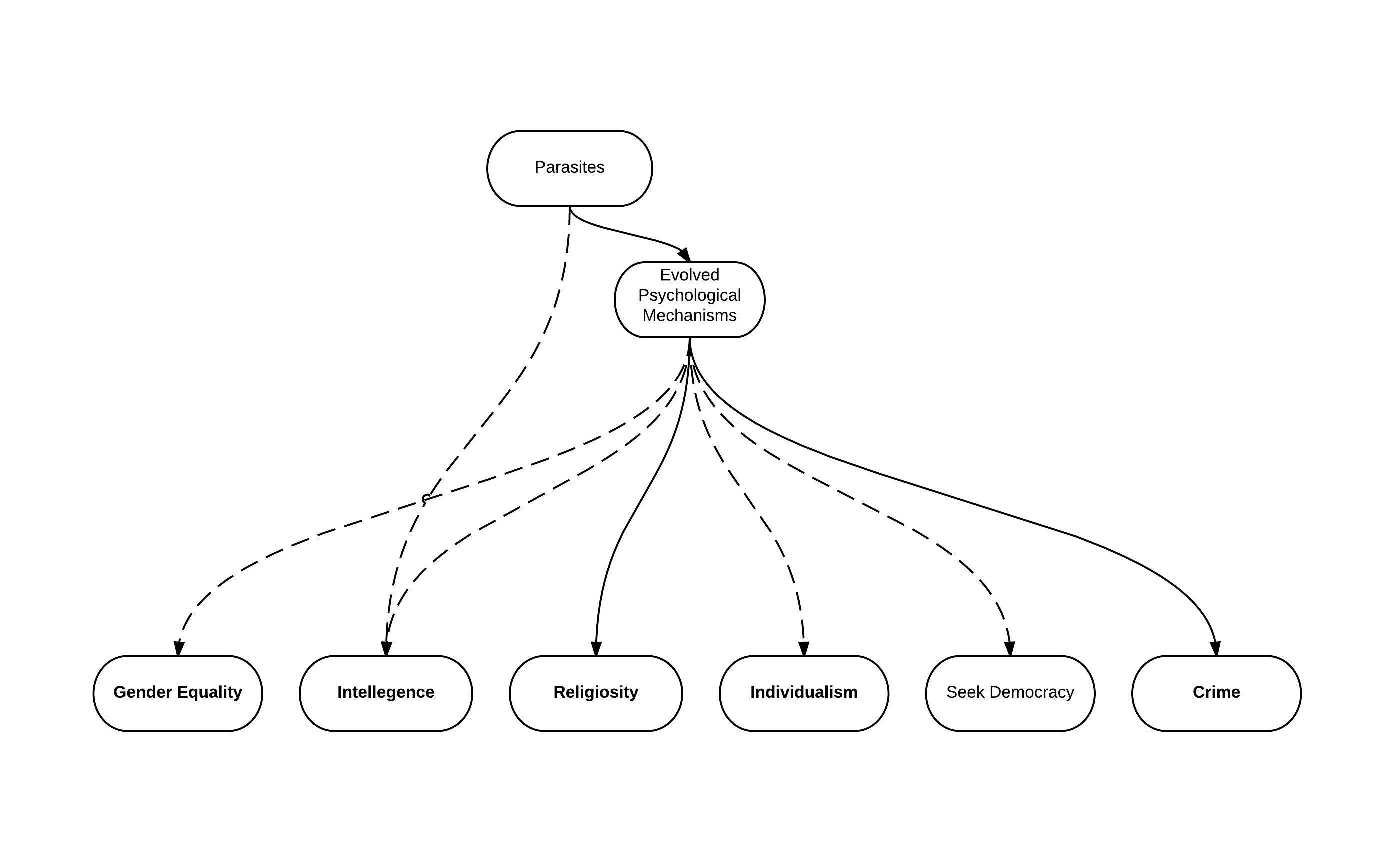
\includegraphics[width=6in]{Figures/NetworkTFE}
        \label{netw:first_sub}
    }
    
        \subfigure[An alternative model, linking structural racism to the outcome variables through various intermediate nodes concerning political economy. This model would also predict correlations between parasite prevalence and many cultural outcomes, but there is no proposed causal role of parasite prevalence on these outcomes.]
    {
        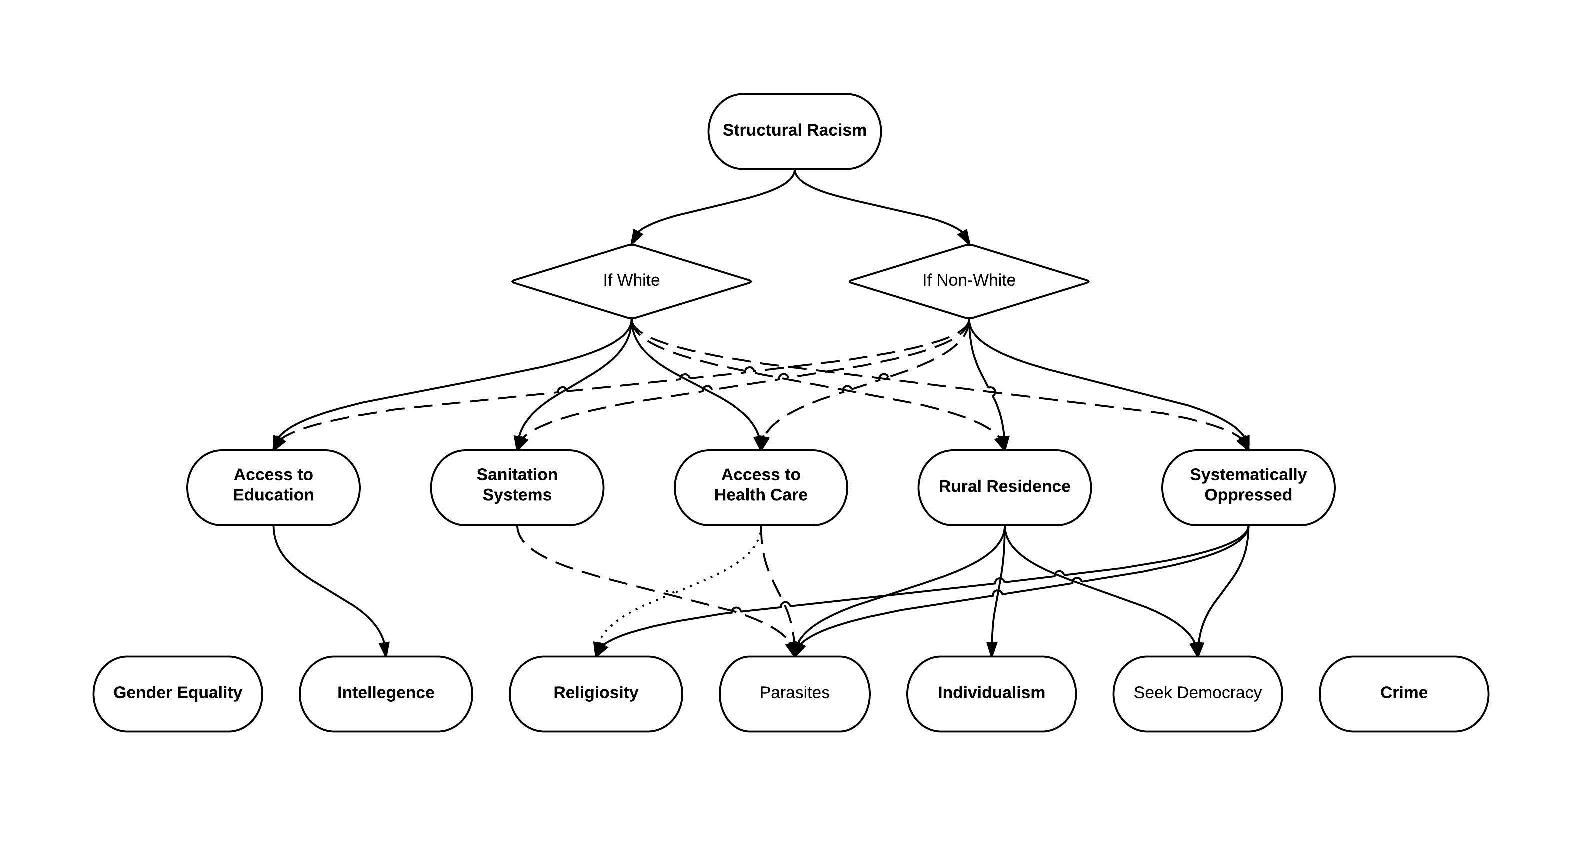
\includegraphics[width=6in]{Figures/NetworkRW}
        \label{netw:second_sub}
    }
\end{figure} 
	
	We must note that the proxies for racism/classism used in this study are indirect, and the outcome variables are self reports; these data could be significantly improved upon by more in-depth research. However, our goal in this study is only to establish the plausibility of alternative hypotheses, and assess their relative strength and cogency in comparison with the parasite models.  More thorough data and more detailed anthropological fieldwork would be required to more securely establish causal relationships between structural racism/classism and cultural characteristics. \\

\noindent\textit{Hypothesis 7: Parasite prevalence in a district is associated with access to sanitation, and sanitation with the ethnic composition of its population}\\

Accordingly, we predict that: (a) there will be a positive association between the existence of sewage and sanitation systems and the proportion of a district that is white, (b) parasite prevalence will be lower in districts where a greater proportion of the population has access to sewage and sanitation systems, and (c) parasite prevalence will be lower in areas where the population is composed of a high proportion of whites.\\

\noindent\textit{Hypothesis 8: Direct associations between parasite prevalence and education are spurious, and are better explained as a result of variables related to ethnicity-based biases in education and sanitation access}\\

 Accordingly, we predict that: (a) parasite prevalence will be negatively associated with highest achieved education at the district level, (b) highest achieved education will be positively associated with the proportion of whites living in a district, (c) highest achieved education will be positively correlated with the existence of sewage and sanitation systems, (d) there will be a positive association between the existence of sewage and sanitation systems and the proportion of a district that is white, and (e)  controlling for the proportion of whites in a district, achieved education will not be associated with parasite prevalence.\\

\noindent\textit{Hypothesis 9: Associations between religiosity and parasite prevalence are driven by omitted variables including ethnicity, sanitation access, and generally increased hardship in high parasite, non-white areas }\\

 Accordingly, we predict that: (a) parasite prevalence will be positively associated with religiosity, (b) religiosity will be negatively associated with the proportion of whites living in a district, and (c) controlling for generalized hardship (using district-level proportion of population that is white), religiosity will not be associated with parasite prevalence.
  
\section{Methods}
In a deliberate departure from statistical practices of TFE (see Discussion), we avoid construction of high-level composite data by making use of the empirical observations unmodified by aggregation or conversion into ratios.  Our statistical modeling is conducted using a fully Bayesian, multi-level modeling framework, with outcome distributions \citep{stan-manual:2013} that are appropriate to each type of outcome data (see below). In each model, we utilize the raw count of individuals (N=170,220) examined for parasite infection and individual-level socio-cultural and demographic data (N=5,558), to estimate: 1) parasite prevalence at the district-level, and 2) the relationship between parasite prevalence and socio-cultural outcomes, in a joint probability framework. 

\subsection{Data Sources}
\subsubsection{Global Neglected Tropical Diseases Database}
	The Global Neglected Tropical Disease (GNTD) database \citep{Hurlimann2011} provides open-access, spatially-resolved data on schistosomiasis and a variety of soil transmitted helminthes, hookworms, roundworms, and other parasites in Africa, the Americas, and other areas.  The data are derived from scientific studies in which persons are sampled from the population and tested for infection status.  We extracted all data from the GNTD database that were geo-referenced to South American countries in the years between 1990 and 2013.  We then filtered this data by parasite species, and within parasite species, pooled data over the 1990-2013 time frame within districts  \cite[i.e. we treat the data from each geographically-localized scientific study as a component of a lower-level cluster in a multi-level cluster sample,][]{hughes1996cluster}.  This gives us the count of individuals screened for infection status within each district and the corresponding count of individuals testing positive for infection. Because the studies in the GNTD database may include multiple disease tests for each individual, pooling data across all species of parasites could lead to poor or biased estimates of parasite prevalence; accordingly, we do not pool data across parasite species.
 
	We were interested, however, in knowing if the prevalence rate of a single parasite species serves as a justifiable proxy for generalized parasite prevalence at the district level.   Accordingly, we estimate the correlation between the prevalence of the parasitic roundworm, \textit{Ascaris lumbricoides} and the whipworm, \textit{Trichuris trichiura}, as these are two of the most common parasitic infections in South America and are the two species of parasite with the densest data in the GNTD database. We use a multi-level Bayesian model (see Supplementary Materials section 1.1 for details) to estimate the prevalence of each parasite, and observe a strong correlation ($\rho= 0.62, \text{PCI95: } 0.48, 0.70$) between the prevalence of each disease type at the district level.\footnote{The symbol $PCI95$ indicates the 95\% equal tail posterior credibility (or confidence) interval. It demarcates the region of the posterior distribution containing the central 95\% of posterior confidence).}  While either disease would serve as a general proxy for parasite prevalence at district level, we elected to use the more abundant data on \textit{Ascaris lumbricoides}. No further models were fit to \textit{Trichuris trichiura} data.

\subsubsection{Latinobarómetero}
	We use individual-level response data from the 2008 Latinobarómetro (LB) public opinion survey.   We extracted individual-level data from all districts in which we had parasite prevalence data. In total, we analyze the responses from 5,558 surveys, distributed over 51 districts in 8 countries. The questions used in our analyses are described in detail in the section \textit{Operationalizing and Testing Predictions}, and the raw data are included in the Supplementary Materials.

\subsection{Hierarchical Bayesian Statistical Modeling}
	Depending on the outcome variable, we use one of three Bayesian models: 1) Categorical outcome variables are modeled using Bayesian multinomial regression on district-level category counts (mathematically equivalent to an individual-level categorical regression model, but more computationally efficient); 2) Ordinal outcome variables are modeled using Bayesian ordered logistic regression; and, 3) Binary outcome variables are modeled using Bayesian Bernoulli regression.

\subsubsection{A Multi-Level Model of Disease Prevalence}
	We estimate the prevalence of parasites, $\theta_{[j]} \in (0,1)$ in each district  $j\in \{1\dots J_c\}$, from the data using binomial likelihoods and a prior, estimated from the data, under two levels of hierarchical partial pooling,\footnote{Hierarchical partial pooling allows information collected in other districts within a country to partially inform the parameter estimates in a focal district, improving inference globally \citep{gelman2006data}.} where, $J_c$ indicates the total number of districts in country, $c$:
\begin{equation}
I_{[j]} \sim \text{Binomial}(T_{[j]},\theta_{[j]})
\end{equation}
 $I_{[j]}$ is the count of district-level positive diagnoses, and $T_{[j]}$ is the district-level count of individuals tested for their disease status.

 Let $\theta_{[j]}$ be defined as the inverse logit transformation of $\Theta_{[j]}\in (-\infty,\infty)$, an unconstrained parameter:
\begin{equation}
\theta_{[j]} = \frac{e^{\Theta_{[j]}}}{1 + e^{\Theta_{[j]}}}
\end{equation}
The $\Theta_{[j]}$ parameters in each country, $c$, are then estimated using a multi-level model structure with country-level priors for the country-specific mean, $\mu_{\Theta_{[c]}}\in (-\infty,\infty)$, and dispersion, $\sigma_{\Theta_{[c]}} \in (-\infty,\infty)$. This model structure partially pools information across districts within countries:
\begin{equation}
\Theta_{[j]} \sim \text{Normal}(\mu_{\Theta_{[c]}},\text{exp}(\sigma_{\Theta_{[c]}}))
\end{equation}
The $\mu_{\Theta_{[c]}}$ and $\sigma_{\Theta_{[c]}}$ parameters are themselves estimated using a multi-level structure with continent-level priors. This model structure partially pools information across countries within the South American continent:
\begin{equation}
\mu_{\Theta_{[c]}} \sim \text{Normal}(M_{\Theta},\Sigma_{\Theta})
\end{equation}
\begin{equation}
\sigma_{\Theta_{[c]}} \sim \text{Normal}(S_{\Theta},\Omega_{\Theta})
\end{equation}
We utilize weakly regularizing priors on the hyperparameters:
\begin{equation}
M_{\Theta} \sim \text{Normal}(0,5)
\end{equation}
\begin{equation}
\Sigma_{\Theta} \sim \text{Cauchy}(0,2.5)T[0,\infty]
\end{equation}
\begin{equation}
S_{\Theta} \sim \text{Normal}(0,5)
\end{equation}
\begin{equation}
\Omega_{\Theta} \sim \text{Cauchy}(0,2.5)T[0,\infty]
\end{equation}
where the symbol, $T[0,\infty]$, indicates truncated support on the positive reals. We then use the full posterior of $\theta_{[j]}$, an optimized estimate of the district-level parasite prevalence rate, as a predictor of the social and cultural outcomes for every individual in district $j$. 

Using raw proportions, such as  $\frac{I_{[j]}}{T_{[j]}}$, as predictor variables, or constructed `data', as in TFE, averages out sample size, fails to propagate uncertainty, and can severely bias statistical outcomes \citep{McDonald2009}. The full Bayesian approach utilized in this model, however, logically quantifies and propagates uncertainty and variation in both parasite prevalence and socio-cultural outcomes through all levels of analysis.

\subsubsection{Categorical Data Analysis}
To estimate the effect of a vector of $D\in\mathbb{N}$ covariates, $X_{[j]}\in \mathbb{R}^D$, on each district-level categorical outcome variable with number of categories equal to $K\in\mathbb{N}$, we use a full Bayesian multinomial regression model, where each outcome variable in each district, $Y_{[j]}\in \mathbb{N}^K$, is a vector composed of the counts of individuals per district who selected each category of a survey question:
\begin{equation}
Y_{[j]} \sim \text{Multinomial}( \phi_{[j]},N_{[j]})
\end{equation}
where:
\begin{equation} N_{[j]} = \sum\limits_{k=1}^K Y^{[k]}_{[j]}
\end{equation}
and $\phi_{[j]}\in\mathbb{R}^K$ is a vector of probabilities of selecting each category, estimated from the data as:
\begin{equation}
\phi_{[j]}=\text{Softmax}( \beta*X_{[j]})
\end{equation}
where: $\beta$ is a $K$ by $D$ matrix of parameters, and $X_{[j]}$ is a vector of covariate data in district $j$. The Softmax function is defined for a $K$-vector like $\phi_{[j]}$ as:
\begin{equation}
\text{Softmax}(\phi_{[j]}) = \left(
\frac{\text{exp}({\phi_{[j]}^{[1]}})}{\sum\limits_{k=1}^K \text{exp}(\phi_{[j]}^{[k]})}
, ... ,
\frac{\text{exp}({\phi_{[j]}^{[K]}})}{\sum\limits_{k=1}^K \text{exp}(\phi_{[j]}^{[k]})}\right)
\end{equation}
and yields a vector in the unit $K$-simplex, which is appropriate to use as the parameter vector for a multinomial distribution. The Softmax function is invariant under adding a constant to each component of its input \citep{stan-manual:2013}, so we fix one category as a reference category, by setting its $\beta$  parameters to zero, which both identifies the remaining parameters and re-frames their interpretation as a comparison between other K-1 categories and the reference category about which we are `pivoting.'  We declare weakly regularizing Gaussian priors on the remaining cells of the $\beta$  matrix; for $d=1\to D$, and $k=1\to (K-1)$: 
\begin{equation}
\beta_{[k,d]} \sim \text{Normal}(0,10)
\end{equation}

\subsubsection{Ordinal Data Analysis}
We estimate the effect of a row vector of $D\in\mathbb{N}$ covariates, $X_{[n]}\in \mathbb{R}^D$, on each outcome variable, $Y_{[n]}\in\{1\dots K\}$, where $n$ indexes individuals, and the number of ordered categories is $K\in \mathbb{N}$, using a full Bayesian ordered logistic regression model. The model is parameterized using a single coefficient vector, $\beta \in \mathbb{R}^D$, and a vector of ordered cut-points, $C \in \mathbb{R}^{(K-1)}$:
\begin{equation}
Y_{[n]} \sim \text{Ordered Logistic}( X_{[n]} * \beta ,C)
\end{equation}
Weakly regularizing priors are specified on the regression coefficients:
\begin{equation}
\beta_{[d]} \sim \text{Normal}(0,10)
\end{equation}
All other parameters are given uniform priors over their support, as implemented in Stan \citep{stan-manual:2013}.
 
\subsubsection{Binary Data Analysis}
We estimate the effect of a row vector of $D\in\mathbb{N}$ covariates, $X_{[n]}\in \mathbb{R}^D$, on each outcome variable $Y_{[n]}\in\{0,1\}$, where $n$ indexes individuals, using a full Bayesian Bernoulli regression model. The model is parameterized using a single coefficient vector, $\beta \in \mathbb{R}^D$. We utilize an inverse logit function to map the linear model onto the unit interval: 
\begin{equation}
Y_{[n]} \sim \text{Bernoulli}( \text{Logit}^{-1}(X_{[n]} * \beta))
\end{equation}
Weakly regularizing priors are specified on the regression coefficients:
\begin{equation}
\beta_{[d]} \sim \text{Normal}(0,10)
\end{equation}

\subsubsection{Hamiltonian Markov Chain Monte Carlo in RStan}
To estimate unknown parameters in our models, we use a variant of Hamiltonian Markov Chain Monte Carlo simulation \citep{hoffman-gelman:2012}. Our Markov chains are coded in templated C++ using the Stan 2.2.0 C++ library \citep{stan-software:2013}, and implemented through the R software environment. In the Supplementary Materials sections 1.1 to 1.14, we thoroughly address model fit, Markov chain convergence diagnostics, and effective posterior sample size for each model fit in this study.  Our data sets and model code are also included in the Supplementary Materials.

\section{Results}
Table \ref{tab1} presents the results for each of the models fit in this paper. We discuss the results specific to each hypothesis in the following paragraphs. Model fit and convergence diagnostics for all of the following hypothesis tests are presented in the Supplementary Materials, sections 1.2 to 1.14. We illustrate the shape of the posterior distribution for each regression line, in each figure below, by plotting one-hundred random realizations from the MCMC simulation. \\
\begin{table}[h]\caption{Regression Estimates. For ease of reference, we provide the slope coefficient(s) for each model fit in this study. Values are the posterior mean and the central 0.95 posterior credibility intervals.}\label{tab1}
\begin{footnotesize}
\begin{tabular}{@{}lllll@{}}
\toprule
\textbf{Hypothesis} & \textbf{Model Outcome}                   & \textbf{\vtop{\hbox{\strut Parasite}\hbox{\strut Prevalence}}} & \textbf{\vtop{\hbox{\strut Sanitation}\hbox{\strut Prevalence}}} & \textbf{\vtop{\hbox{\strut Population Ratio}\hbox{\strut of Whites}}} \\ \midrule
Hypothesis 1        & \textit{Democracy }          &                              &                                &                                     \\
                    & Democracy vs. Indifference               & 2.12 (2.02, 2.39)     & $\cdot$                        & $\cdot$                             \\
                    & Authoritarian vs. Indifference           & -0.30 (-0.85, 0.28)   & $\cdot$                        & $\cdot$                             \\
                    &                                          &                              &                                &                                     \\
Hypothesis 2        &  Market vs. State & 0.28 (0.03, 0.53)     & $\cdot$                        & $\cdot$                             \\
                    &                                          &                              &                                &                                     \\
Hypothesis 3        & Perceived Gender Equality                & 0.15 (-0.13, 0.43)    & $\cdot$                        & $\cdot$                             \\
                    &                                          &                              &                                &                                     \\
Hypothesis 4        & Achieved Education                       & -0.88 (-1.15, -0.61) & $\cdot$                        & $\cdot$                             \\
                    &                                          &                              &                                &                                     \\
Hypothesis 5        & Violent Crime                            & 0.02 (-0.29, 0.31)   & $\cdot$                        & $\cdot$                             \\
                    &                                          &                              &                                &                                     \\
Hypothesis 6        & Religiosity                             & 0.59 (0.15, 0.89)     & $\cdot$                        & $\cdot$                             \\
                    &                                          &                              &                                &                                     \\
Hypothesis 7(a)     & \textit{Ethnicity}                                &                              &                                &                                     \\
                    & Indigenous vs. White                     & 6.60 (5.71, 7.49)     & $\cdot$                        & $\cdot$                             \\
                    & Black vs. White                          & 8.66 (7.59, 9.71)     & $\cdot$                        & $\cdot$                             \\
                    & Mulato vs. White                         & 7.32 (6.18, 8.46)     & $\cdot$                        & $\cdot$                             \\
                    & Mestizo vs. White                        & 8.87 (8.16, 9.6)      & $\cdot$                        & $\cdot$                             \\
                    &                                          &                              &                                &                                     \\
Hypothesis 7(b)     & Parasite Prevalence                      & $\cdot$                      & -4.37 (-4.75, -4.23)    & $\cdot$                             \\
                    &                                          &                              &                                &                                     \\
Hypothesis 7(c)     & \textit{Ethnicity }                               &                              &                                &                                     \\
                    & Indigenous vs. White                     & $\cdot$                      & -20.65 (-23.67, -18.03) & $\cdot$                             \\
                    & Black vs. White                          & $\cdot$                      & -6.01 (-8.02, -4.21)    & $\cdot$                             \\
                    & Mulato vs. White                         & $\cdot$                      & -5.95 (-7.90, -4.16)    & $\cdot$                             \\
                    & Mestizo vs. White                        & $\cdot$                      & -11.54 (-13.53, -9.90)  & $\cdot$                             \\
                    &                                          &                              &                                &                                     \\
Hypothesis 8(c)     & Achieved Education                       & $\cdot$                      & $\cdot$                        & 1.00 (0.83, 1.18)           \\
Hypothesis 8(d)     & Achieved Education                       & -0.17 (-0.46, 0.12)  & $\cdot$                        & 0.95 (0.78, 1.14)            \\
                    &                                          &                              &                                &                                     \\
Hypothesis 9(b)     & Religiosity                             & $\cdot$                      & $\cdot$                        & -1.13 (-1.34, -0.90)        \\
Hypothesis 9(c)     & Religiosity                             & -0.21 (-0.54, 0.10)  & $\cdot$                        & -1.20 (-1.40, -0.99)         \\ \bottomrule
\end{tabular}
\end{footnotesize}
\end{table}


\subsection{Tests of Association Between Parasite Prevalence and Socio-Cultural Characteristics}
\noindent\textit{Hypothesis 1 Result:  Parasite prevalence is positively associated with preferences for democracy}

	Contrary to \citet{Thornhill2009}, we find that parasite prevalence is positively and reliably associated with preferences for democracy, $\beta=2.12$ (PCI95: 2.02, 2.39), and negatively associated with preferences for authoritarianism, $\beta=-0.30
$ (PCI95: -0.85, 0.28), relative to the indifference  response (``for people like me, it doesn't matter'').  Figure \ref{resDem} plots the posterior distributions of the probability of selecting one of the three categorical responses as a function of parasite prevalence. There is an overall preference for democracy relative to authoritarianism, but this ratio grows from about 3 to 1 in low parasite districts, to 8 to 1 in high parasite districts.   
 \begin{figure}
\caption{\label{resDem}  Posterior distributions of the probability of selecting categorical responses as a function of parasite prevalence.  We see that: 1) preference for authoritarianism decline as a function of increasing parasite prevalence [in units of frequency $\in (0,1)$ ]; 2) preference for democracy increase as a function of increasing parasite prevalence; and, 3) indifference/apathy toward the political system grow relative to preference for authoritarianism as parasite prevalence in a district increases.  }
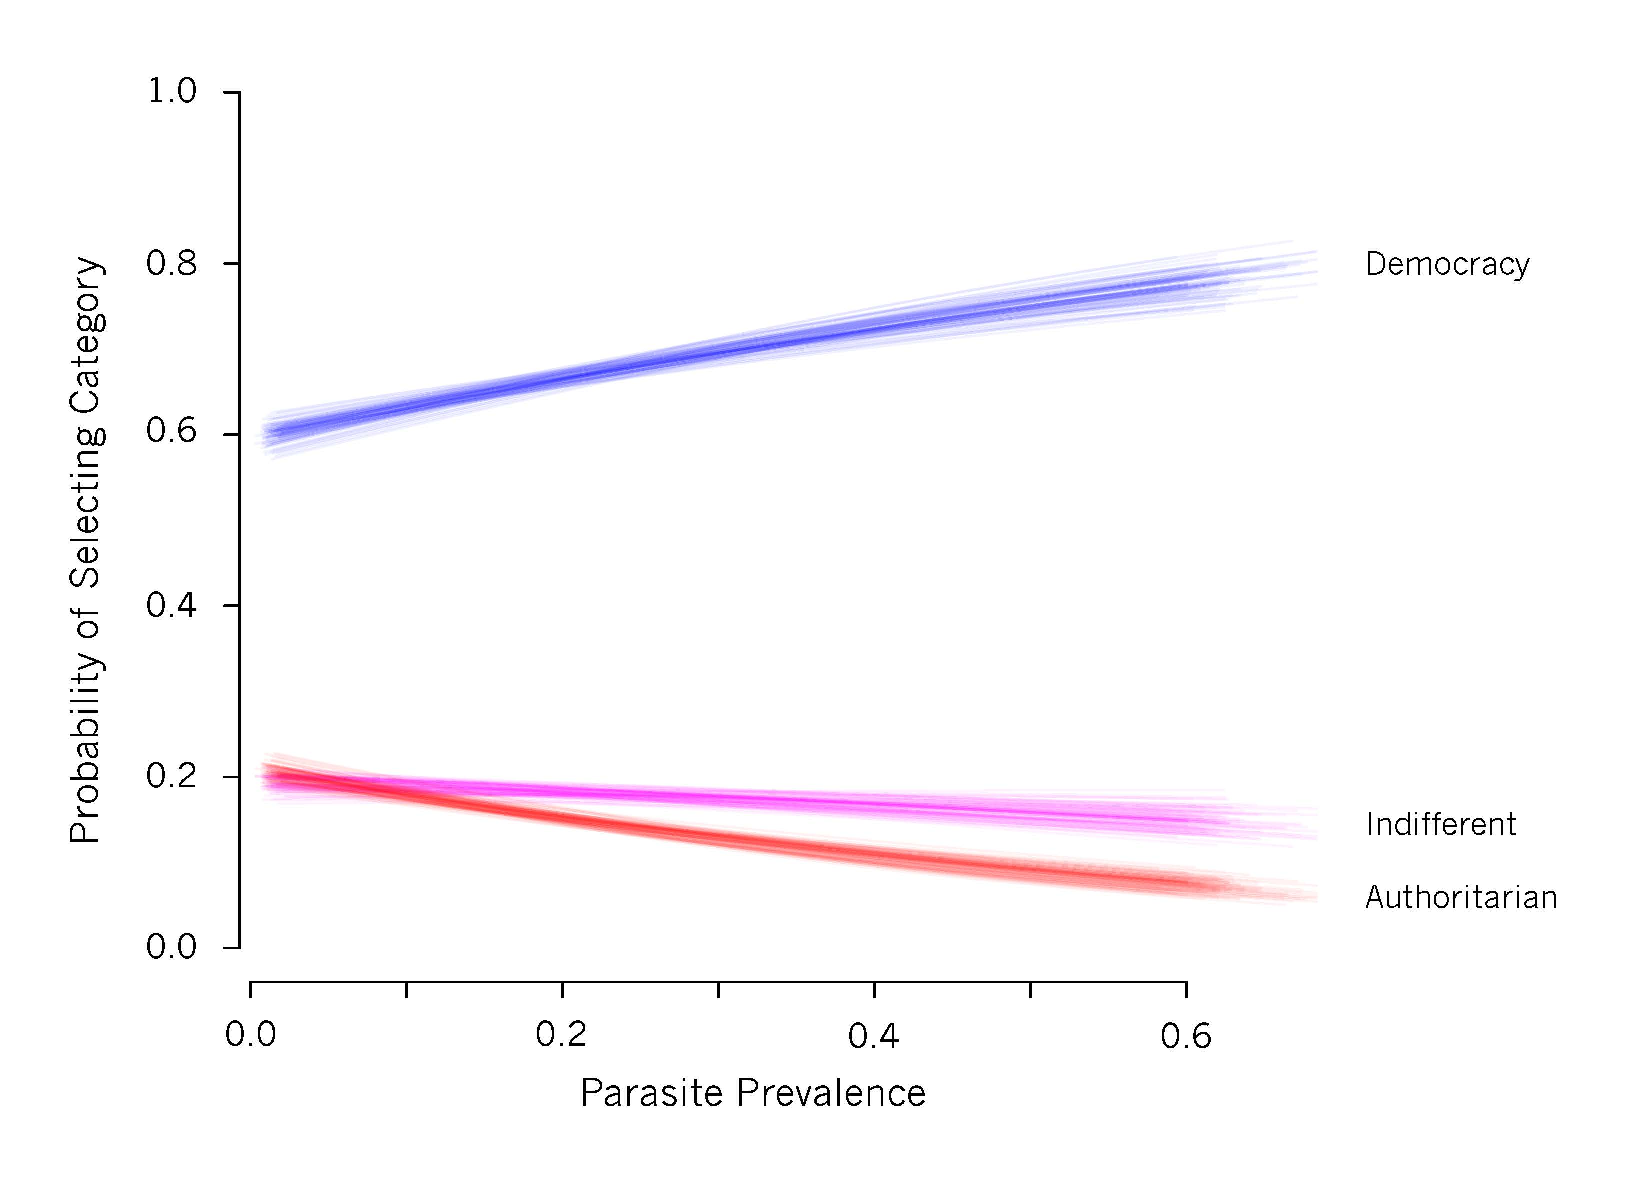
\includegraphics[width=5in]{Figures/DemocracyModel} 
\end{figure}

\noindent\textit{Hypothesis 2 Result: Parasite prevalence is negatively associated with collectivism}

	Contrary to \citet{Thornhill2009}, parasite prevalence is positively associated with preferences for individualism and negatively associated with preferences for collectivism.  The absolute value of the effect is small but reliable, $\beta=0.28$ (PCI95: 0.03, 0.53). Figure \ref{resCol} plots the results of ordered categorical regression modeling.\\
 \begin{figure}
\caption{\label{resCol}  Posterior distributions of the cumulative probability of an individual responding below a given ordered categorical threshold on the 1 to 10 scale measuring preference for state or free market solutions, respectively.  As red shifts to blue, preferences shift from the market fixing/controlling economic problems (individualism) to the state fixing/controlling of economic problems (collectivism). Each group of lines corresponds to one of the ordered categorical responses available to respondents, plotted as a function of parasite prevalence.  We find that: 1) the majority of the population, regardless of parasite prevalence, favors state control of economic issues, as the majority of the cumulative probability density is accounted for by the responses corresponding to increased state control; 2) the response profiles vary only slightly as a function of parasite prevalence; and, 3) to the minor extent that increased parasite prevalence varies with social preferences on the individualism/collectivism spectrum, it varies positively with preferences for market individualism, as can be seen by the slightly downward sloping lines (from left to right), which indicate that more cumulative probability is accounted for by higher item rankings (free market preferences) when parasite prevalence is high. }
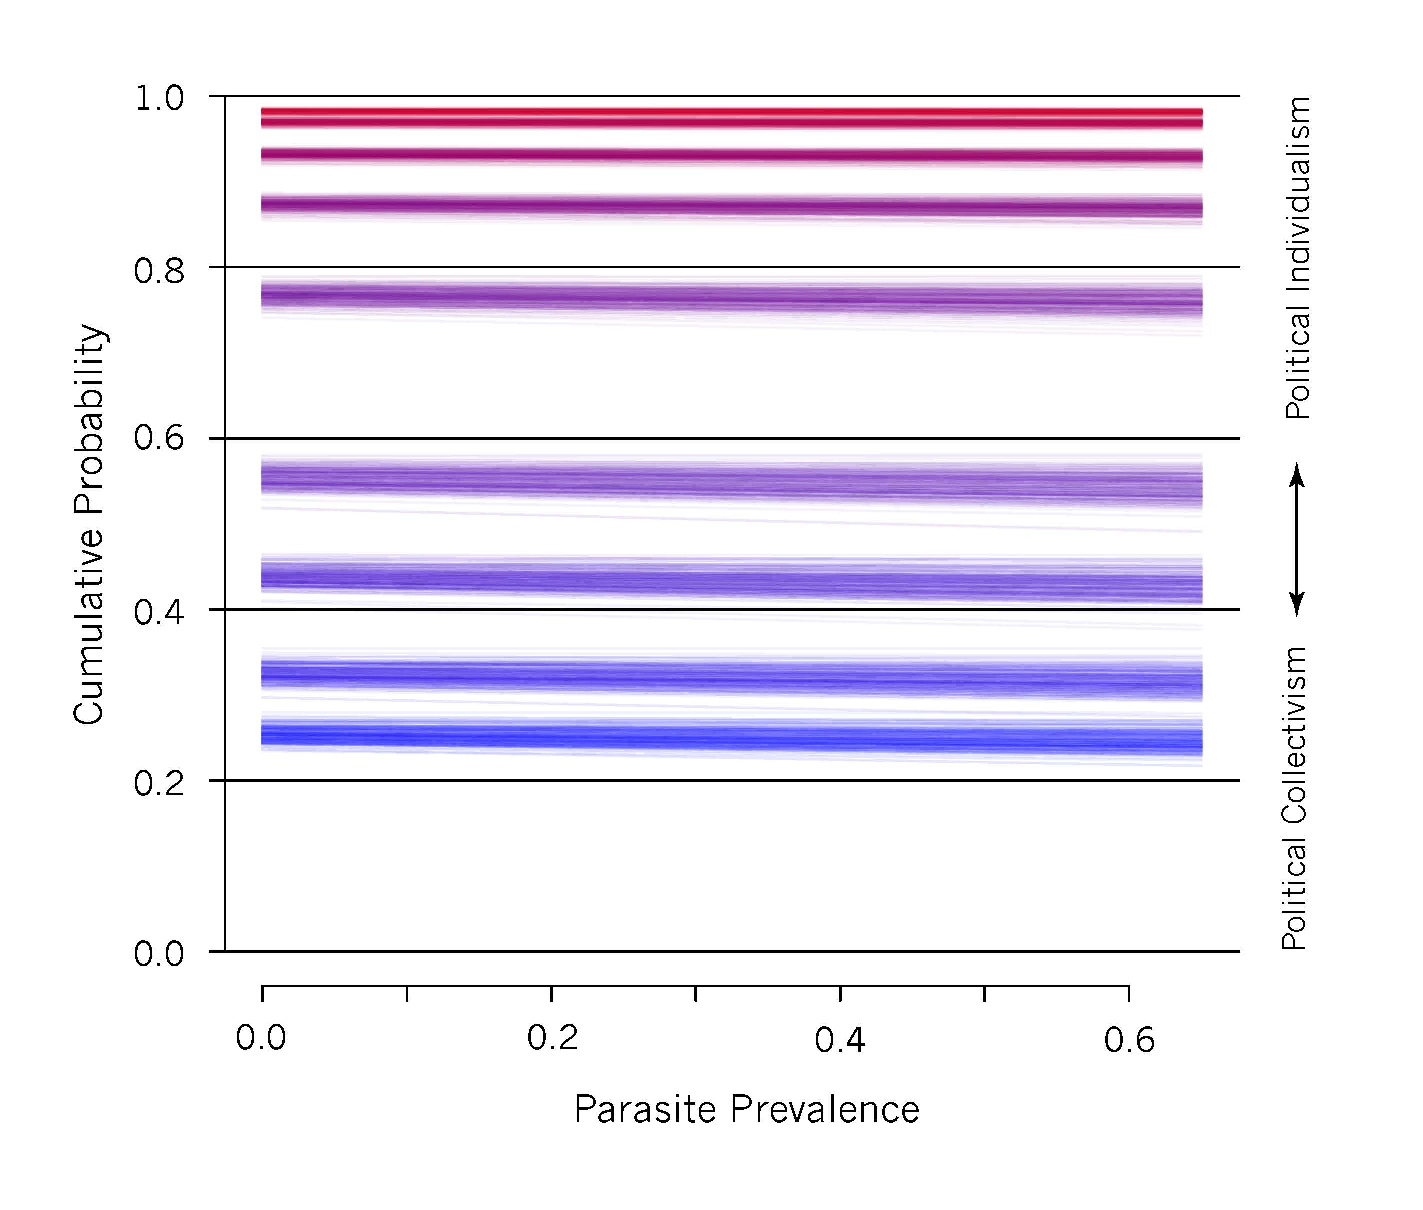
\includegraphics[width=5in]{Figures/CollectivismModel} 
\end{figure}

	
\noindent\textit{Hypothesis 3 Result: Parasite prevalence is positively, but not reliably, associated with gender equality}

	Contrary to the findings of \citet{Thornhill2009}, we find no evidence that parasite prevalence is negatively associated with gender equality at the district level, $\beta=0.15$ (PCI95: -0.13, 0.43).  Figure \ref{resGen} plots the results of ordered categorical regression modeling.\\
 \begin{figure}
\caption{\label{resGen}  Posterior distributions of the cumulative probability of an individual responding below a given ordered categorical threshold. As red shifts to blue, individuals report an increasing equality of men and women, from ``Not at All,'' to ``Fully.'' We find that: 1) across districts about 18\% of respondents think that equality of men and women is never ensured (``Not at all''), and 20\% of respondents think it is always ensured (``Fully''), with the majority of the population falling somewhere in between; 2) there is almost no variation in gender equality as a function of parasite prevalence across districts; and, 3) to the extent that any difference in gender equality exists as a function of parasite prevalence, there is a slight but non-reliable trend towards increased gender equality in districts where parasite prevalence is high. }
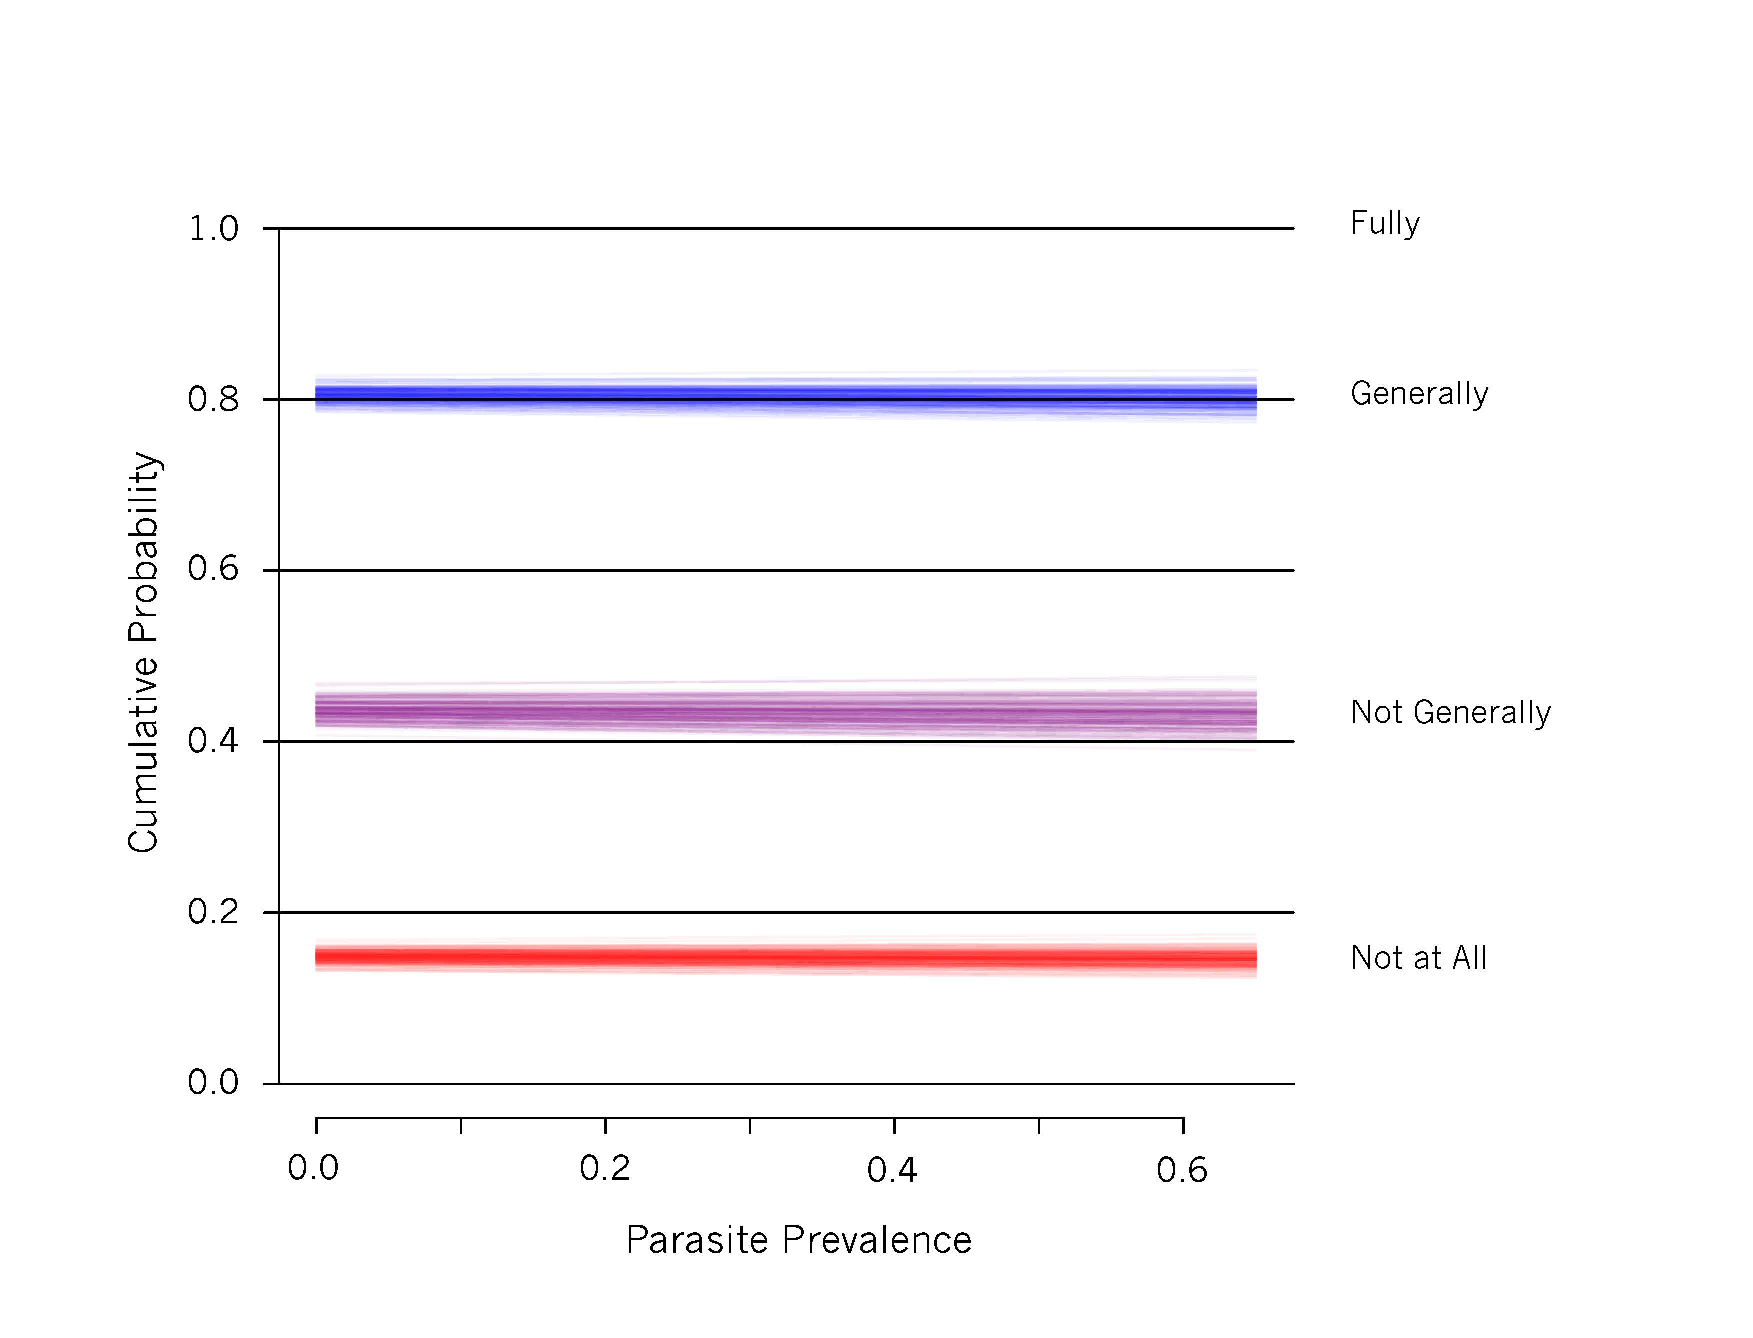
\includegraphics[width=5in]{Figures/GenderEqualityModel} 
\end{figure}

\noindent\textit{Hypothesis 4 Result: Parasite prevalence is negatively associated with educational achievement}

	As predicted in \citet{Eppig2010}, we find evidence that total achieved education is negatively associated with parasite prevalence, $\beta=-0.88$ (PCI 95: -1.15, -0.61). However, this effect appears to be driven by lack of access to secondary or higher education in high parasite areas (see Figure \ref{resEdu}), not by lack of educational attainment in primary school or early childhood as was predicted by \citet[][pg2]{Eppig2010}. \\
 \begin{figure}
\caption{\label{resEdu}  Posterior distributions of the cumulative probability of an individual achieving below a given ordered categorical threshold of education. As red shifts to blue, individuals report an increasing level of achieved education. Each group of lines corresponds to one of the ordered categorical responses available to respondents (0 years through 12 years of primary/secondary education, plus 3 ordered classes of post-secondary education), plotted as a function of parasite prevalence.  We can see that: 1) across districts, approximately equal levels of primary education are achieved, regardless of parasite prevalence (this is shown by the cluster of categorical thresholds for which Cumulative Probability $<0.2$); 2) there is evidence of slightly lower educational achievement as a function of increasing parasite prevalence for secondary school levels of education (this is shown by the cluster of categorical thresholds for which Cumulative Probability $>0.3$ and $<0.7$); and, 3) there are only slight differences in higher educational achievement as a function of parasite prevalence (this is shown by the cluster of categorical thresholds for which Cumulative Probability $>0.8$).}
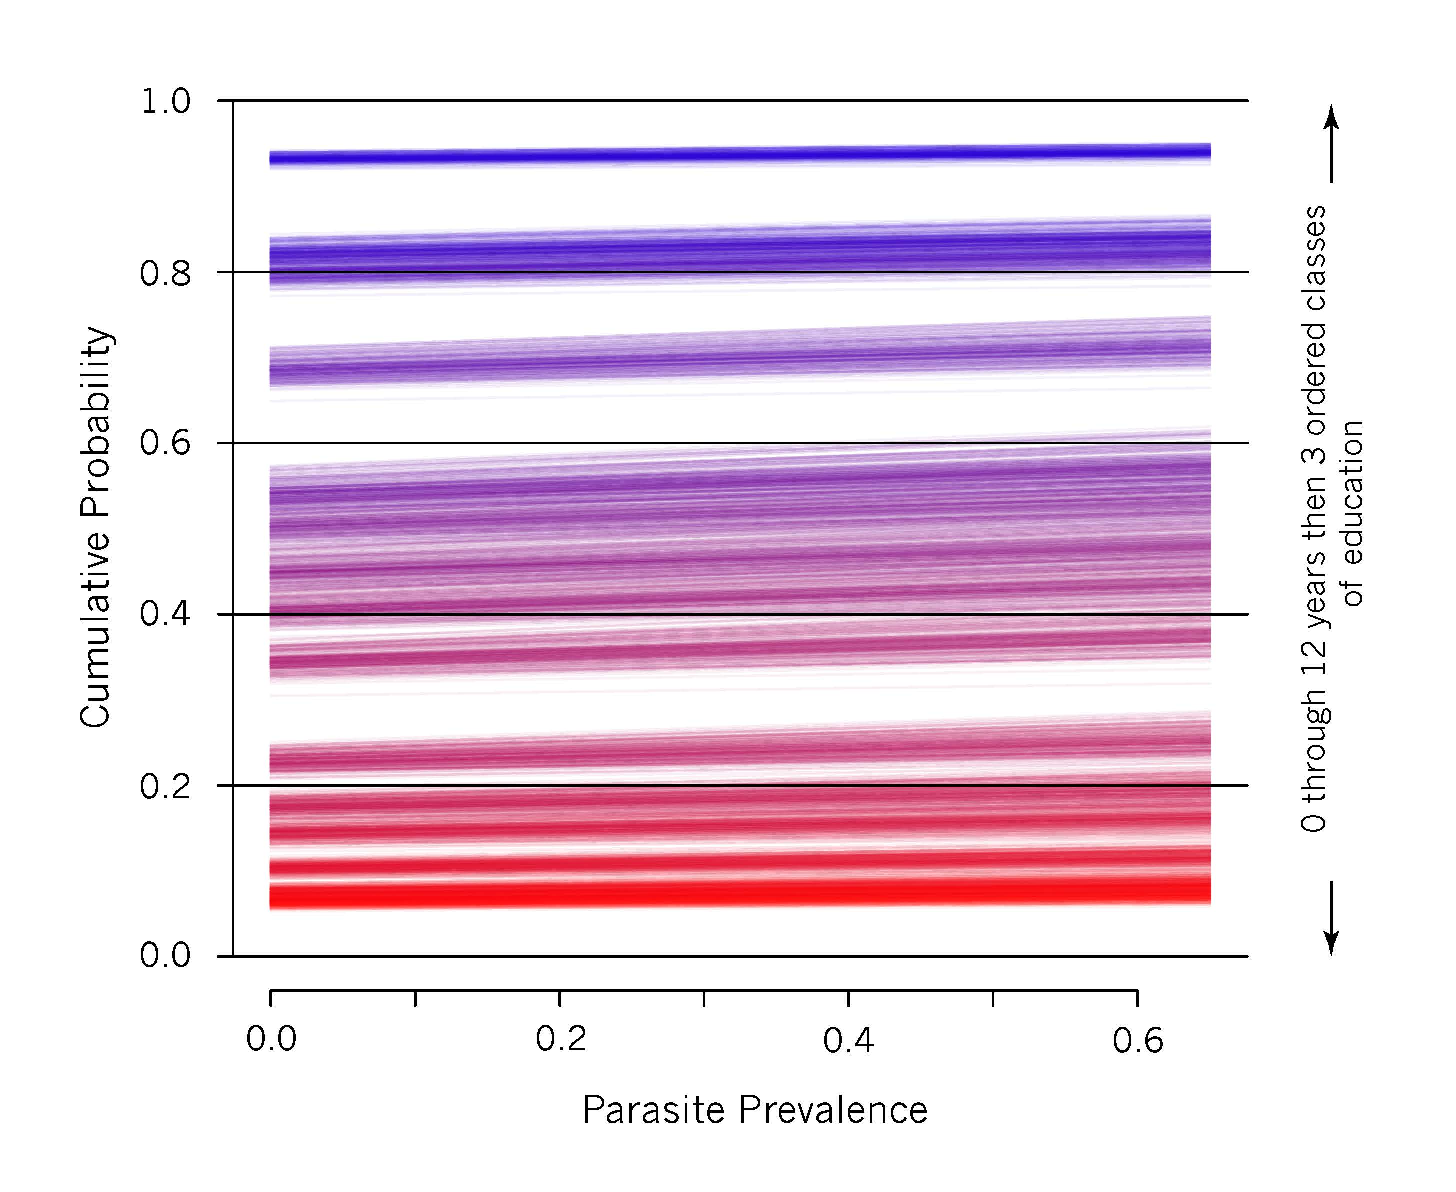
\includegraphics[width=5in]{Figures/EducationModel} 
\end{figure}  

\noindent\textit{Hypothesis 5 Result: Parasite prevalence is not associated with violent crimes}

	Contrary to \citet{Thornhill2011}, we find no evidence that parasite prevalence is associated with the frequency of violent crimes, $\beta=0.02$ (PCI 95: -0.29, 0.31). Figure \ref{resViolence} shows that the regression of a respondent (or an immediate family member of the respondent) being the victim of an assault, attack, or crime, on parasite prevalence is almost perfectly flat, indicating no reliable effect.\\
 \begin{figure}
\caption{\label{resViolence}  Posterior distribution of the regression of a respondent (or an immediate family member of the respondent) being the victim of an assault, attack, or crime, on parasite prevalence. The Y axis is probability of experiencing an assault, attack, or crime.  The data show no relationship between the prevalence of parasites and violent crime.}
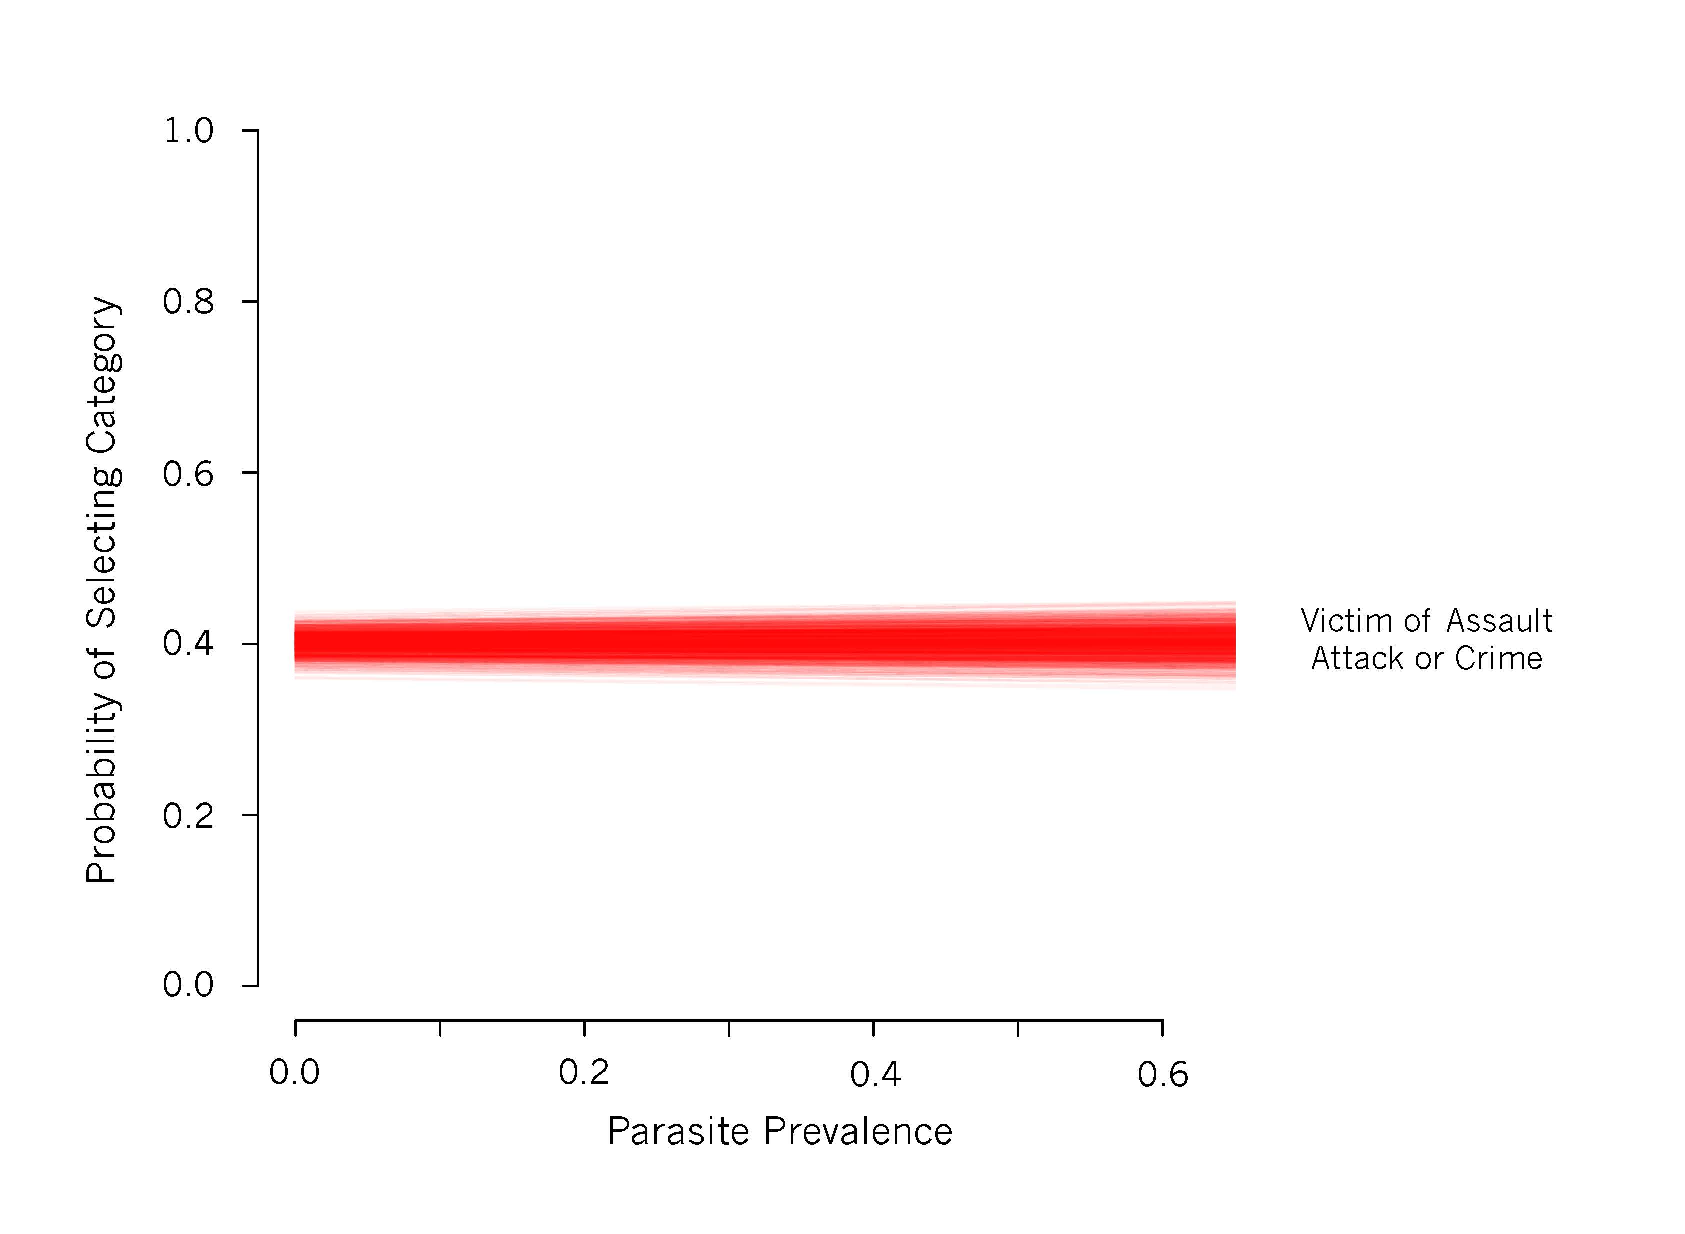
\includegraphics[width=5in]{Figures/ViolenceModel} 
\end{figure}  


\noindent\textit{Hypothesis 6 Result: Parasite prevalence is positively associated with religiosity}

	As in \citet{Fincher2012}, we find evidence that religiosity is positively associated with parasite prevalence, $\beta=0.59$ (PCI95: 0.15, 0.89). As shown in Figure \ref{resRel}, however, the absolute effect size is small (about $2.5\%$ as one moves from parasite-free regions to high parasite regions).\\
 \begin{figure}
\caption{\label{resRel}  Posterior distributions of the cumulative probability of an individual responding below a given ordered categorical threshold. As blue shifts to red, individuals report an increasing level of religiosity. The bottom-most group of blue lines is the posterior distribution of the cut-point between those with ``No Religion,'' and those with religions (but with varying levels of religiosity). Every other group of lines corresponds to the posterior distribution of one of the other ordered categorical responses available to respondents describing their level of religiosity, plotted as a function of parasite prevalence. We find that:  1) across districts there is almost no variation in the proportion of the population with ``No Religion,'' as a function of parasite prevalence; 2) there is almost no variation in the proportion of the population that self identifies as ``Very Devout,'' as a function of parasite prevalence across districts; and, 3) to the extent that any differences in religiosity exist as a function of parasite prevalence, there is a slight trend for individuals in high parasite regions to mark ``Devout'' as opposed to ``Not very devout,'' when describing their religiosity (the absolute value of this effect as one moves from parasite-free regions to high parasite regions is about $2.5\%$). }
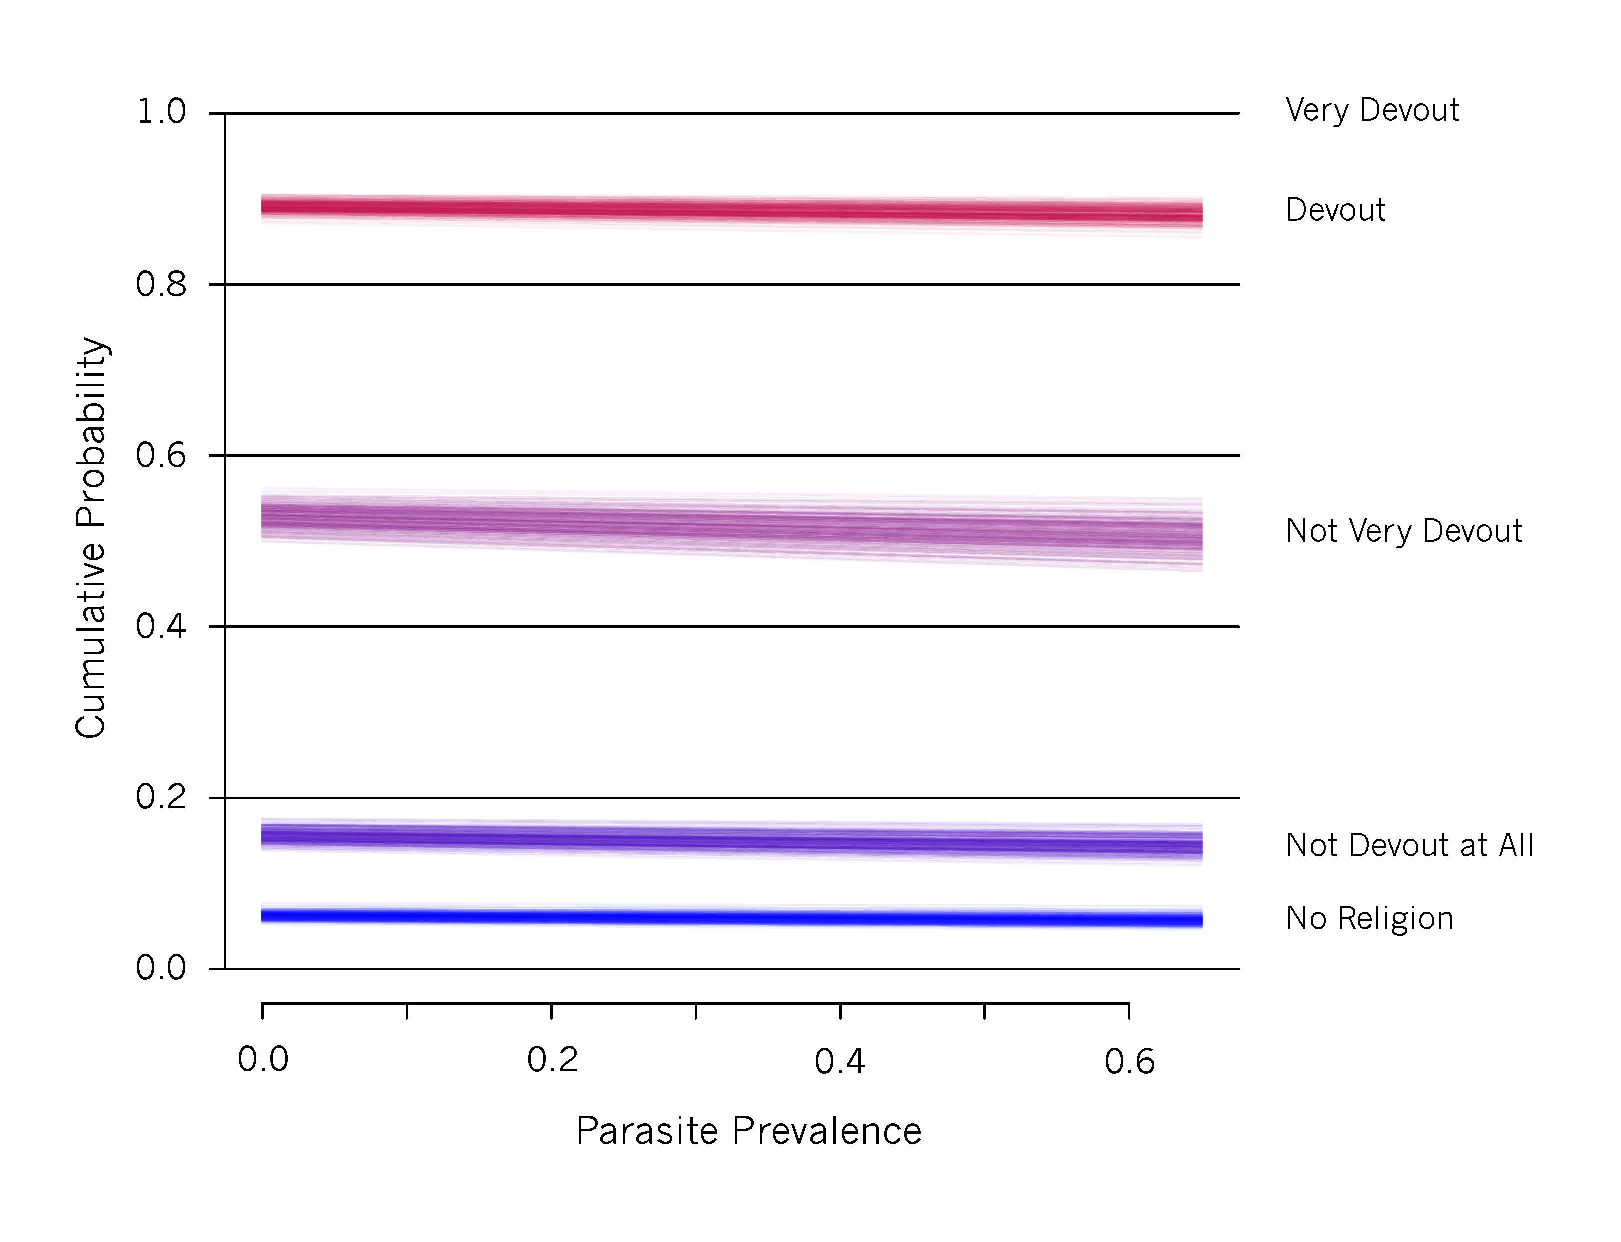
\includegraphics[width=5in]{Figures/ReligiosityModel} 
\end{figure}

\subsection{Structural Racism, Sanitation, and Socio-Cultural Characteristics}
\noindent\textit{Hypothesis 7 Results: District racial/ethnic composition is strongly associated with sanitation improvements and parasite prevalence}

	There is a strong positive association of the district-level population ratios of peoples of color and parasite prevalence: $\beta_{Indigenous}=6.60$ (PCI95: 5.71, 7.49), $\beta_{Black}=8.66$ (PCI95: 7.59, 9.71), $\beta_{Mulato}=7.32$ (PCI95: 6.18, 8.46), and $\beta_{Mestizo}=8.87$ (PCI95: 8.16,  9.6) ($\beta$ values are relative to $\beta_{White}$). The likelihood of a randomly selected individual being a person of color in a high parasite district is more than 6 times as large as the likelihood of a randomly selected individual being a person of color in a parasite-free district. To visualize these results on the probability scale, we plot the fraction of the population by ethnicity as a function of parasite prevalence in Figure \ref{resStructRacism}.\\

 \begin{figure}
\caption{\label{resStructRacism}  Posterior distributions of the fraction of the population by ethnicity as a function of parasite prevalence. We find that: 1) the majority of the population across districts identify as either white or mestizo, with individuals identifying as black, indigenous, or mulato comprising only a small fraction of the population; 2) individuals identifying as white compose the majority of the population in parasite-sparse or parasite-free districts and compose a small fraction of the population in high-parasite districts; 3) individuals identifying in one of the non-white categories compose a small fraction of the population in parasite-sparse districts, but an increasing fraction of the population as parasite prevalence at the district level increases.}
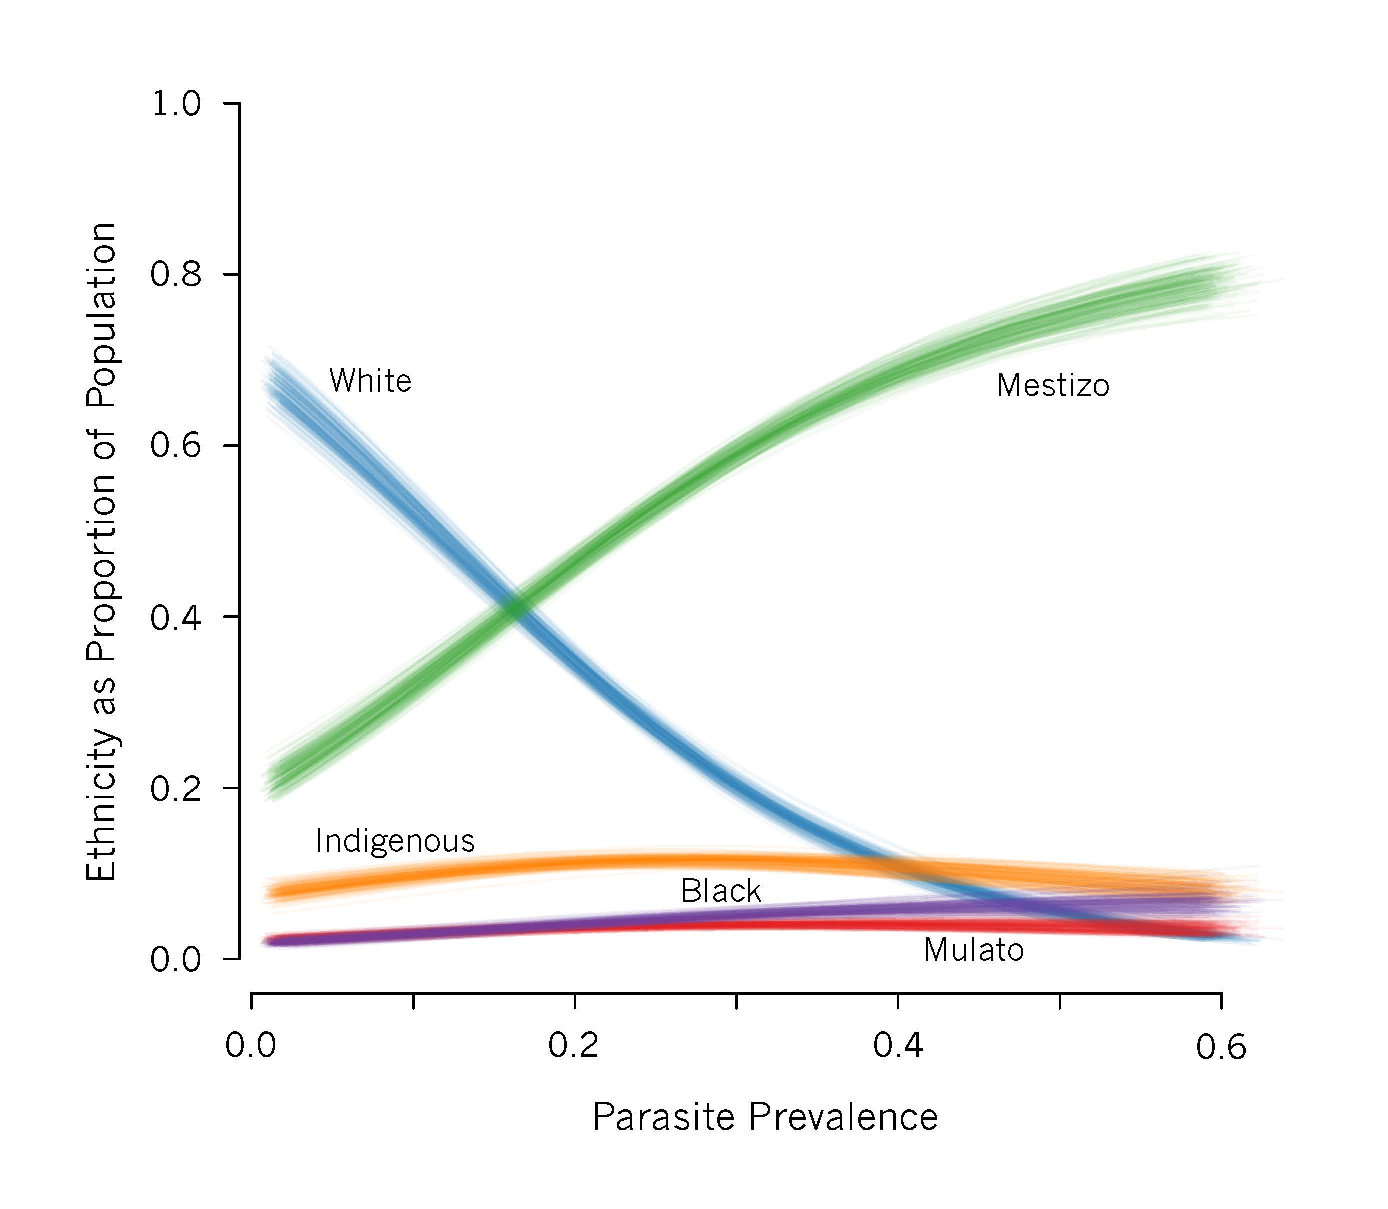
\includegraphics[width=5in]{Figures/StructuralRacismModel} 
\end{figure}

Likewise, we find strong evidence that the prevalence of parasites is negatively associated with the presence of sewage and sanitation systems, $\beta=-4.37$ (PCI95:$ -4.75, -4.23$). Figure \ref{resSewer} plots the result.\\
 \begin{figure}
\caption{\label{resSewer} Posterior distributions of the regression line linking parasite prevalence and the presence sewage and sanitation systems. From this plot, we can see that: 1) as parasite prevalence increases in a district, we observe a co-occurring decrease in access to sanitation systems.}
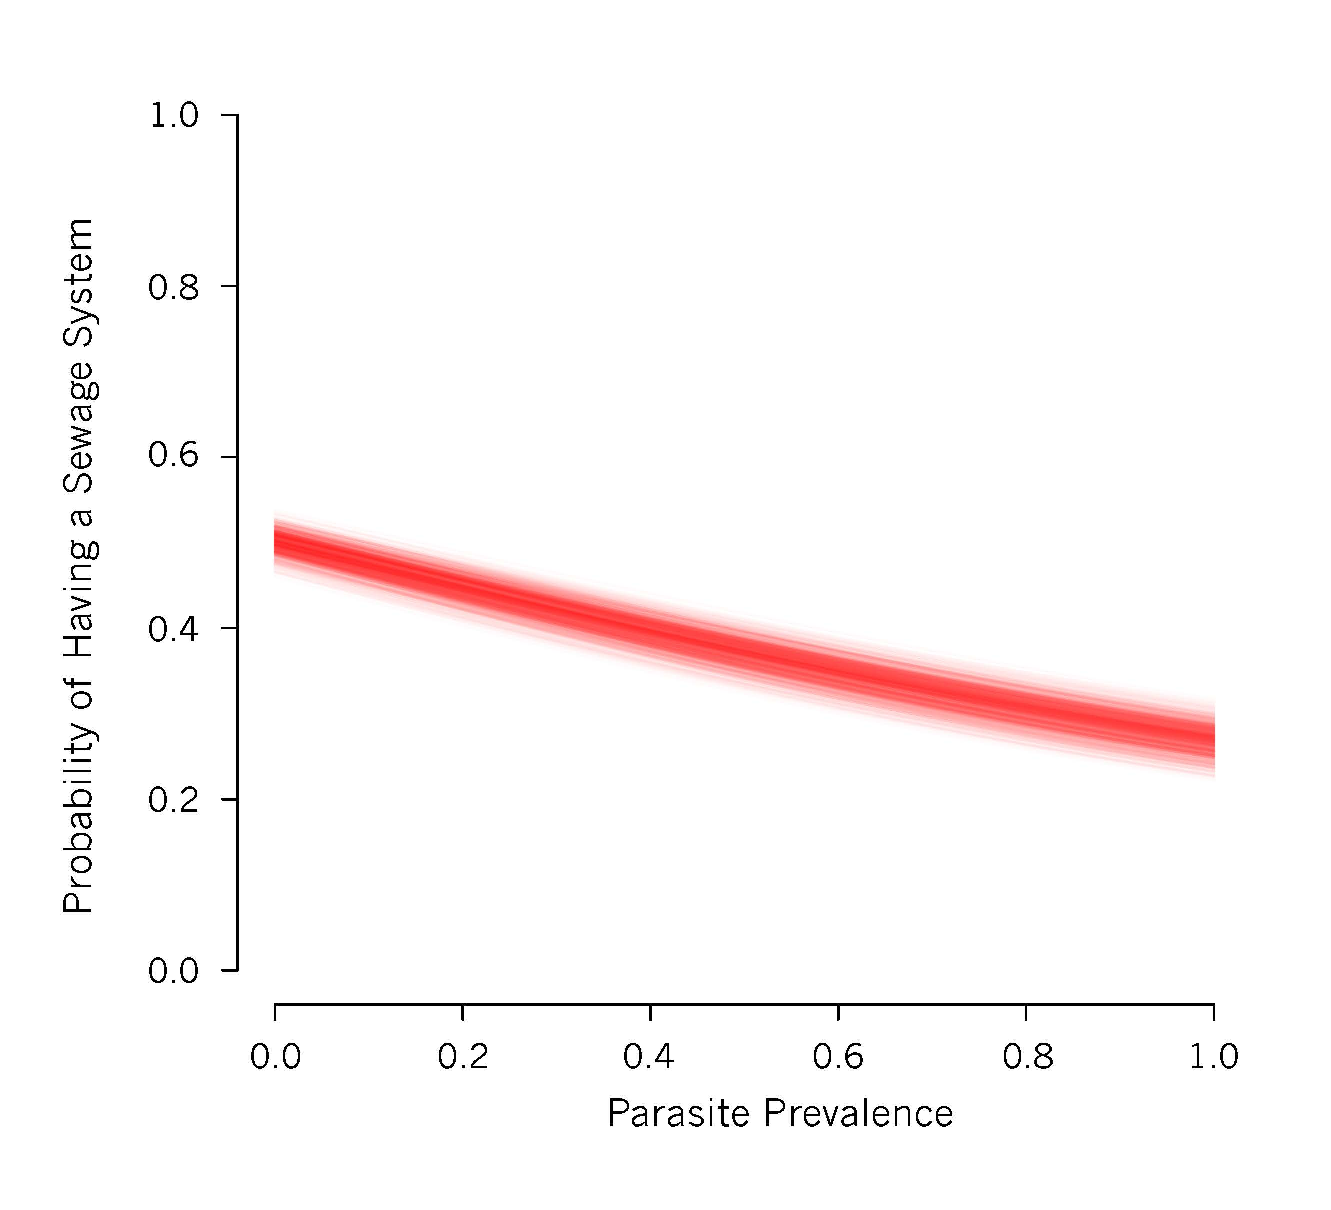
\includegraphics[width=5in]{Figures/SewerModel} 
\end{figure}

Finally, we find strong evidence that the prevalence of sewage and sanitation systems is negatively associated with the proportion of individuals in a district that are people of color, $\beta_{Indigenous}=-20.65$ (PCI95: -23.67, -18.03), $\beta_{Black}=-6.01$ (PCI95: -8.02, -4.21), $\beta_{Mulato}=-5.95$ (PCI95: -7.90, -4.16), and $\beta_{Mestizo}=-11.54
$ (PCI95: -13.53,  -9.90) ($\beta$ values are relative to $\beta_{White}$). Figure \ref{resSewerEth} plots these results. All-white or nearly-all-white districts are the only ones with universal or near-universal sanitation.\\
 \begin{figure}
\caption{\label{resSewerEth} Posterior distributions of the fraction of the population by ethnicity as a function of the fraction the population with sewage and sanitation services. We can see that: 1) areas with near universal sewage and sanitation services are composed almost entirely of whites; 2) areas with intermediate levels of sewage and sanitation service are primarily composed of mestizo and whites (with the white portion of the district presumably having greater access to such services); and, 3) areas with diminished access to sewage and sanitation services are primarily composed of indigenous populations.}
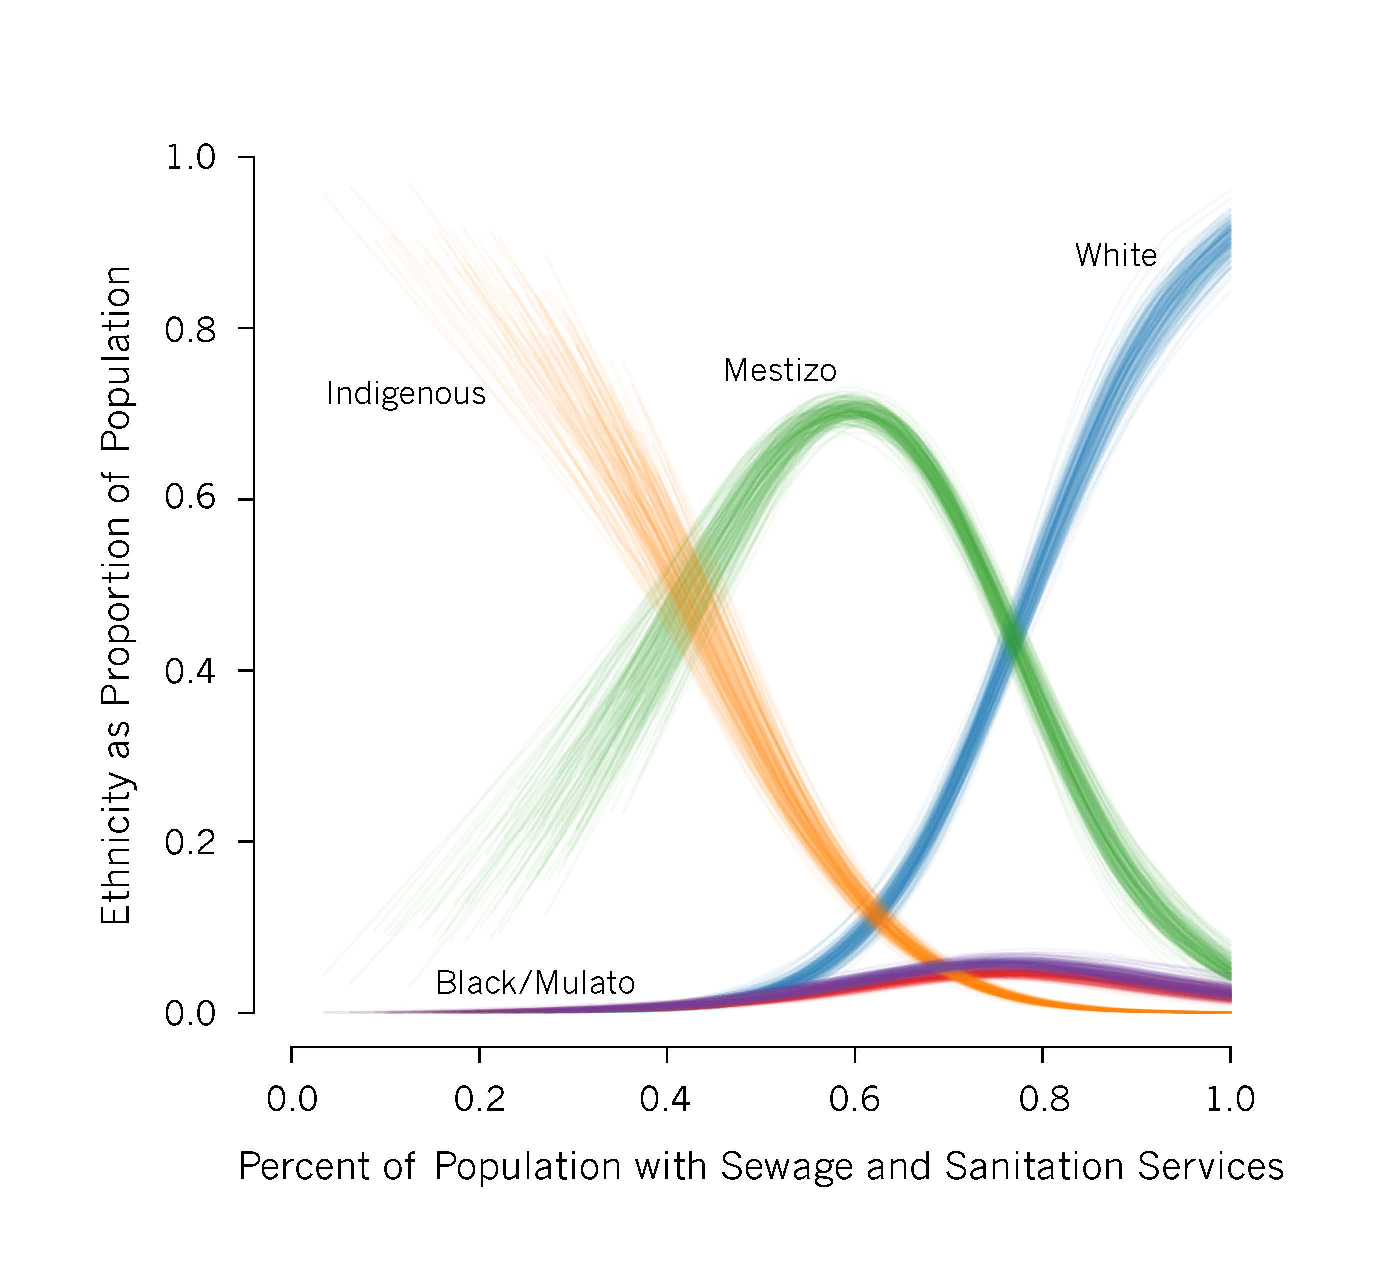
\includegraphics[width=5in]{Figures/SewageAndEthnicityModel} 
\end{figure}

\noindent\textit{Hypothesis 8 Results (Our Retest of Hypothesis 4):  Association between parasite prevalence and achieved education is an artifact of district-level racial/ethnic composition}
	
	We find evidence that achieved education is negatively associated with parasite prevalence (see Hypothesis 4). However, we also find that increasing the percentage of whites in a district is positively associated with the existence of sewage and sanitation systems (see Hypothesis 7). Finally, we find that achieved level of education is positively associated with the proportion of population that is white, $\beta=1.00$ (PCI 95: 0.83, 1.18). Figure \ref{resWhiteEdu} plots the results.\\
 \begin{figure}
\caption{\label{resWhiteEdu} Posterior distributions of the cumulative probability of an individual achieving below a given ordered categorical threshold of education.  As red shifts to blue, individuals report an increasing level of achieved education. Each group of lines corresponds to one of the ordered categorical responses available to respondents, plotted as a function of the district level proportion of whites. We find that: 1) there is a strong effect of the proportion of population that is white on increasing achieved education, an effect stronger than the effect of parasite prevalence on education (as seen in Figure \ref{resEdu}).}
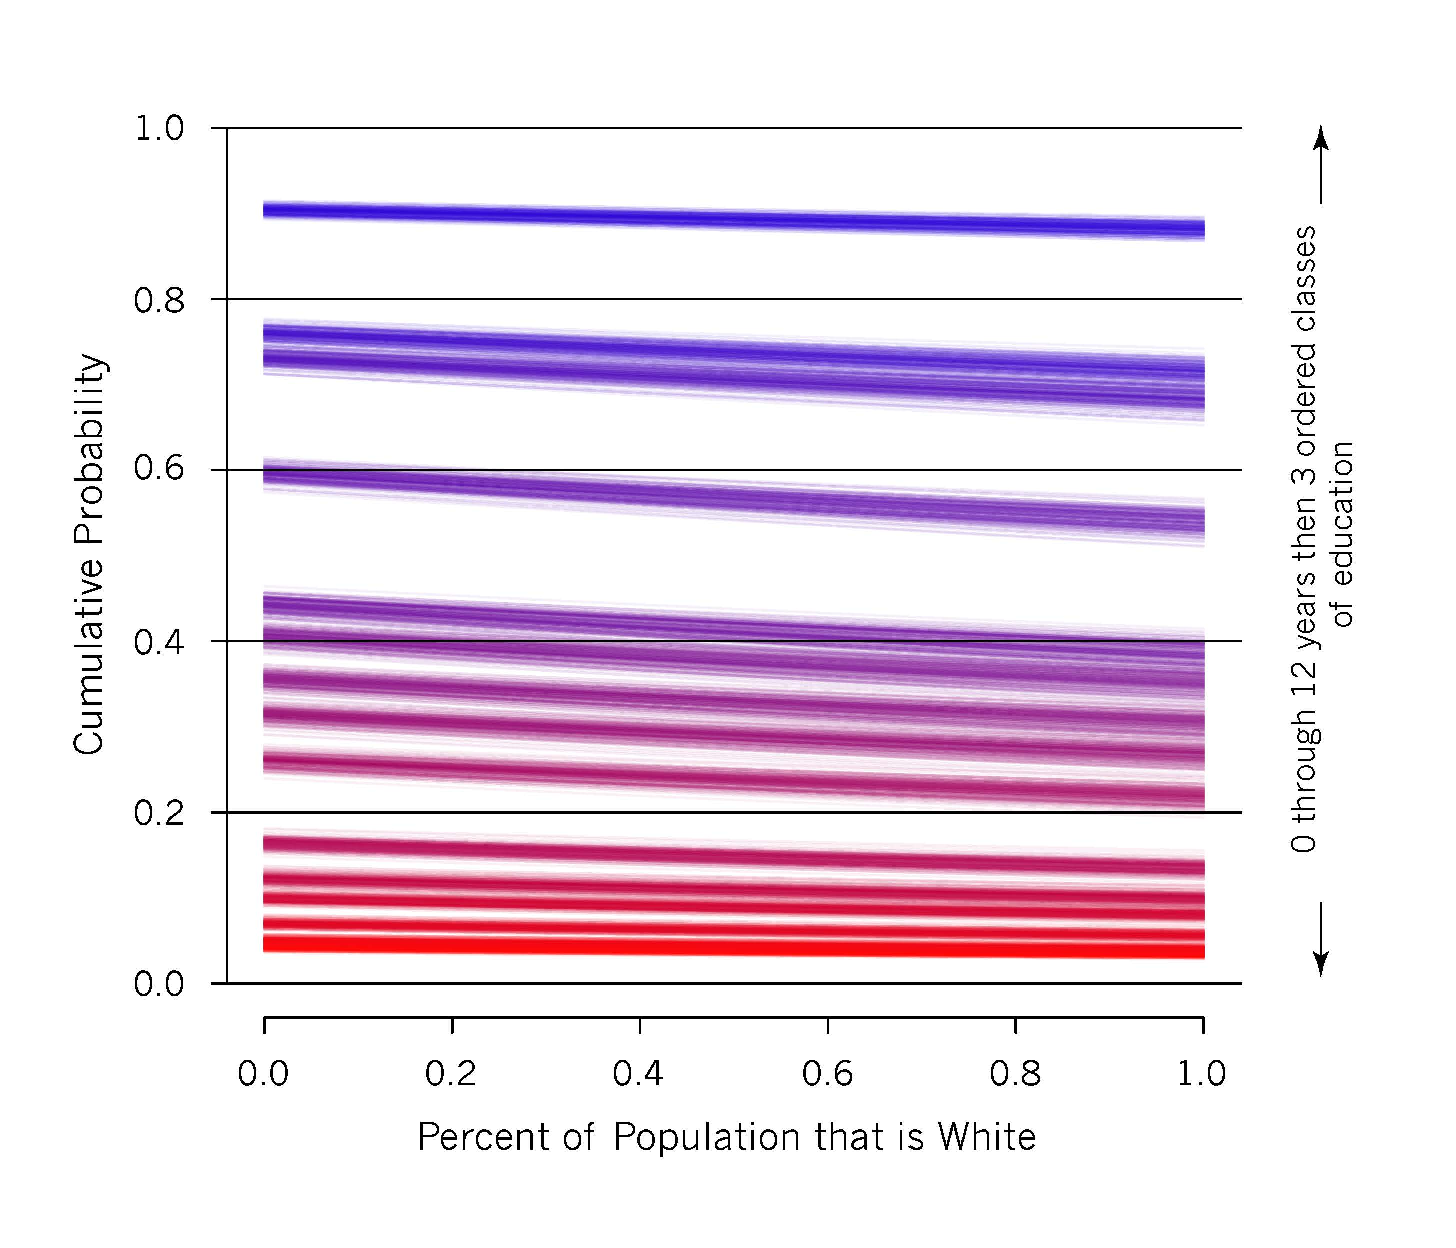
\includegraphics[width=5in]{Figures/WhiteEducationModel} 
\end{figure}  

	These findings suggest that the inverse relationship between parasite prevalence and educational achievement is not necessarily causal and is likely an artifact of district racial/ethnic composition (with elevated white population ratios being associated with greater provisioning of sanitation, lower frequency of parasites and, independently of parasites, elevated funding for education and thus educational achievement). When both district-level racial/ethnic composition and parasite prevalence are used to predict educational achievement in a multiple regression model, parasite prevalence ceases to be a reliable predictor, $\beta_{parasite}=-0.17
$, (PCI 95: -0.46, 0.12), while the proportion of whites in the population remains a reliable predictor, $\beta_{whitness}=0.95$, (PCI95: 0.78, 1.14). Figure \ref{ALubWhiteEdu} plots the results.\\
\begin{figure}
    \centering
    \caption {Posterior distributions of the cumulative probability of an individual achieving below a given ordered categorical threshold of education. Frame (a) plots the posterior distribution of achieved eduction as a function of parasite prevalence, when a district is composed of all non-whites; Frame (b) plots the posterior distribution of achieved education as a function of parasite prevalence, when a district is composed of all whites. Each group of lines corresponds to one of the ordered categorical responses available to respondents (years of education), plotted as a function of district-level parasite prevalence. As red shifts to blue, individuals report an increasing level of achieved education. We find that: 1) there is a strong effect of the proportion of population that is white on increasing achieved education (about a 20\% increase in achieving a secondary school education); and, 2) controlling for the proportion of a district that is white, there is no effect of parasite prevalence on education.}  \label{ALubWhiteEdu}
    \subfigure[Frame (a) plots the model posterior when a district has a population with no whites.]
    {
        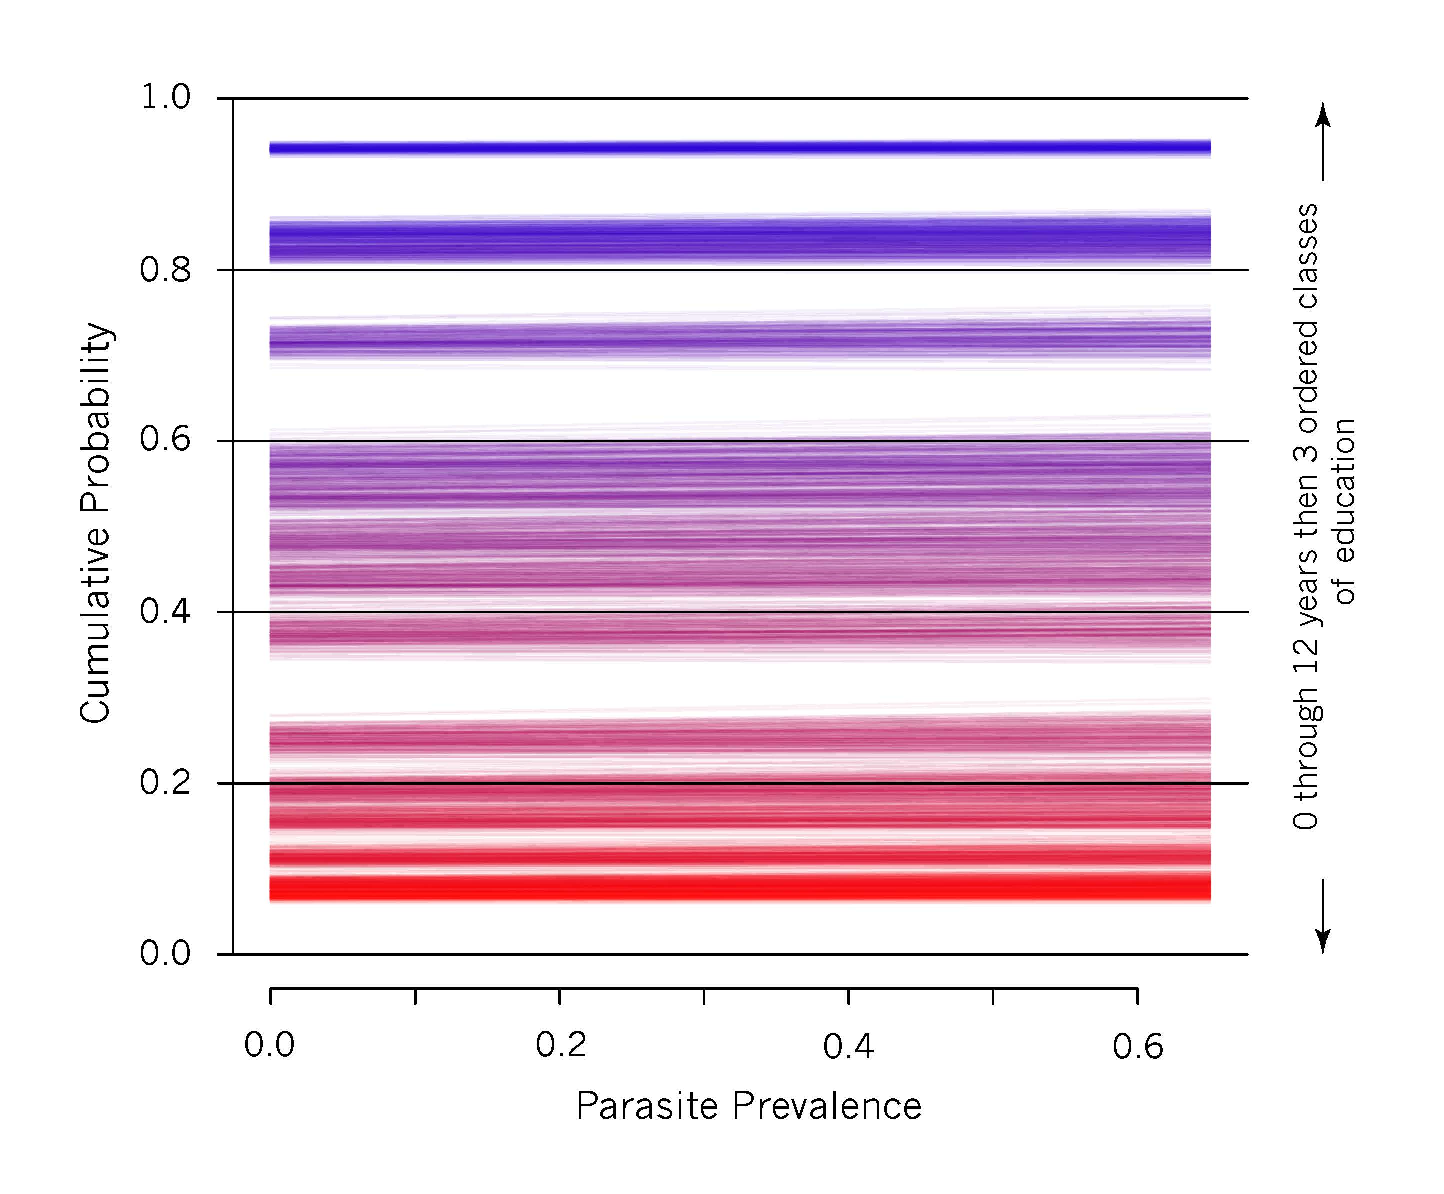
\includegraphics[width=3in]{Figures/WhiteEducationModel(WhiteEquals0)}
        \label{ALubWhiteEdu:first_sub}
    }     \subfigure[Frame (b) plots the model posterior when a district has a population that is all white. ]
    {
        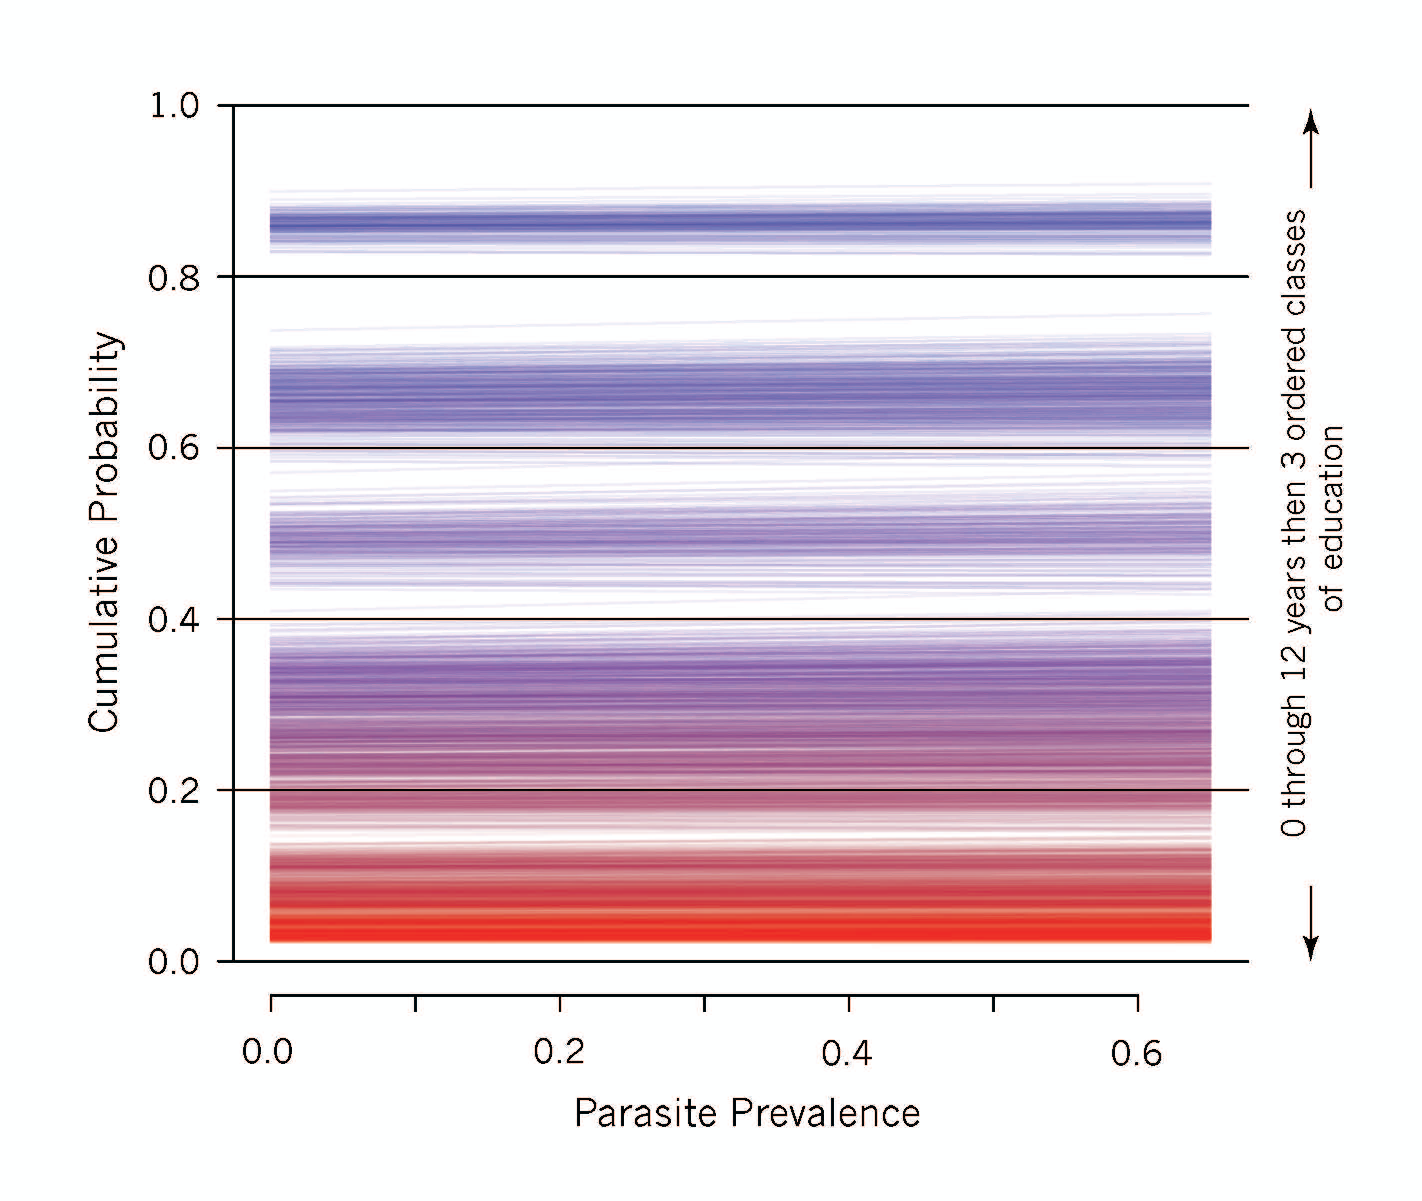
\includegraphics[width=3in]{Figures/WhiteEducationModel(WhiteEquals1)}
        \label{ALubWhiteEdu:second_sub}
    }
\end{figure} 

\noindent\textit{Hypothesis 9 Results (Our Retest of Hypothesis 6): The association between parasite prevalence and religiosity is likely an artifact of factors associated with district-level racial/ethnic composition}

	We find evidence that religiosity is positively associated with parasite prevalence (Hypothesis 6). However, existing literature provides reason to believe that this relationship would be expected given the well known proximate mechanism linking hardship, suffering, and medical problems to increased religiosity \citep{koenig2001religion}. Given the increased hardship of non-white populations relative to the white population in terms of health outcomes and access to sewage and sanitation systems, we fit a model regressing religiosity on the district-level proportion of whites.  We find that religiosity is inversely associated with the proportion of population that is white (a proxy for access to essential services like water, sewage and sanitation services, and medical care), $\beta=-1.13$, (PCI 95:  -1.34, -0.90).\\  
	
	We know from Hypothsis 8 that the district-level proportion of population that is white is a valid proxy for access to  sewage and sanitation services.  When the proportion of population that is white and parasite prevalence are used to predict religiosity in a multiple regression model, parasite prevalence ceases to be a reliable predictor of religiosity, $\beta_{parasite}=-0.21 $, (PCI 95: -0.54, 0.10), while the proportion of population that is white remains a strong predictor, $\beta_{whitness}= -1.20$, (PCI95: -1.40, -0.99). Figure \ref{ALubWhitenessAndReligModel} plots the results.\\
\begin{figure}
    \centering
    \caption {Figure \ref{ALubWhitenessAndReligModel} plots the posterior distributions of the cumulative probability of an individual responding below a given ordered categorical threshold. As blue shifts to red, individuals report an increasing level of religiosity. Frame (a) plots the model posterior when a district has a population with no whites; Frame (b) plots the model posterior when a district has a population that is all white. The bottom-most group of blue lines is the posterior distribution of the cut-point between those with ``No Religion,'' and those with religions (but with varying levels of religiosity). Every other group of lines corresponds to the posterior distribution of one of the other ordered categorical responses available to respondents describing their level of religiosity, plotted as a function of parasite prevalence.  The main results of the multiple regression model is that: 1) there are strong baseline differences in religosity as a function of the proportion whites in a district (a proxy measure for decreased access to essential services like water, sewage and sanitation services, and medical care); and, 2) there is essentially no variation in religiosity as a function parasite prevalence, controlling for the proportion of whites in a district. }  \label{ALubWhitenessAndReligModel}
    \subfigure[Frame (a) plots the model posterior when a district has a population with no whites.]
    {
        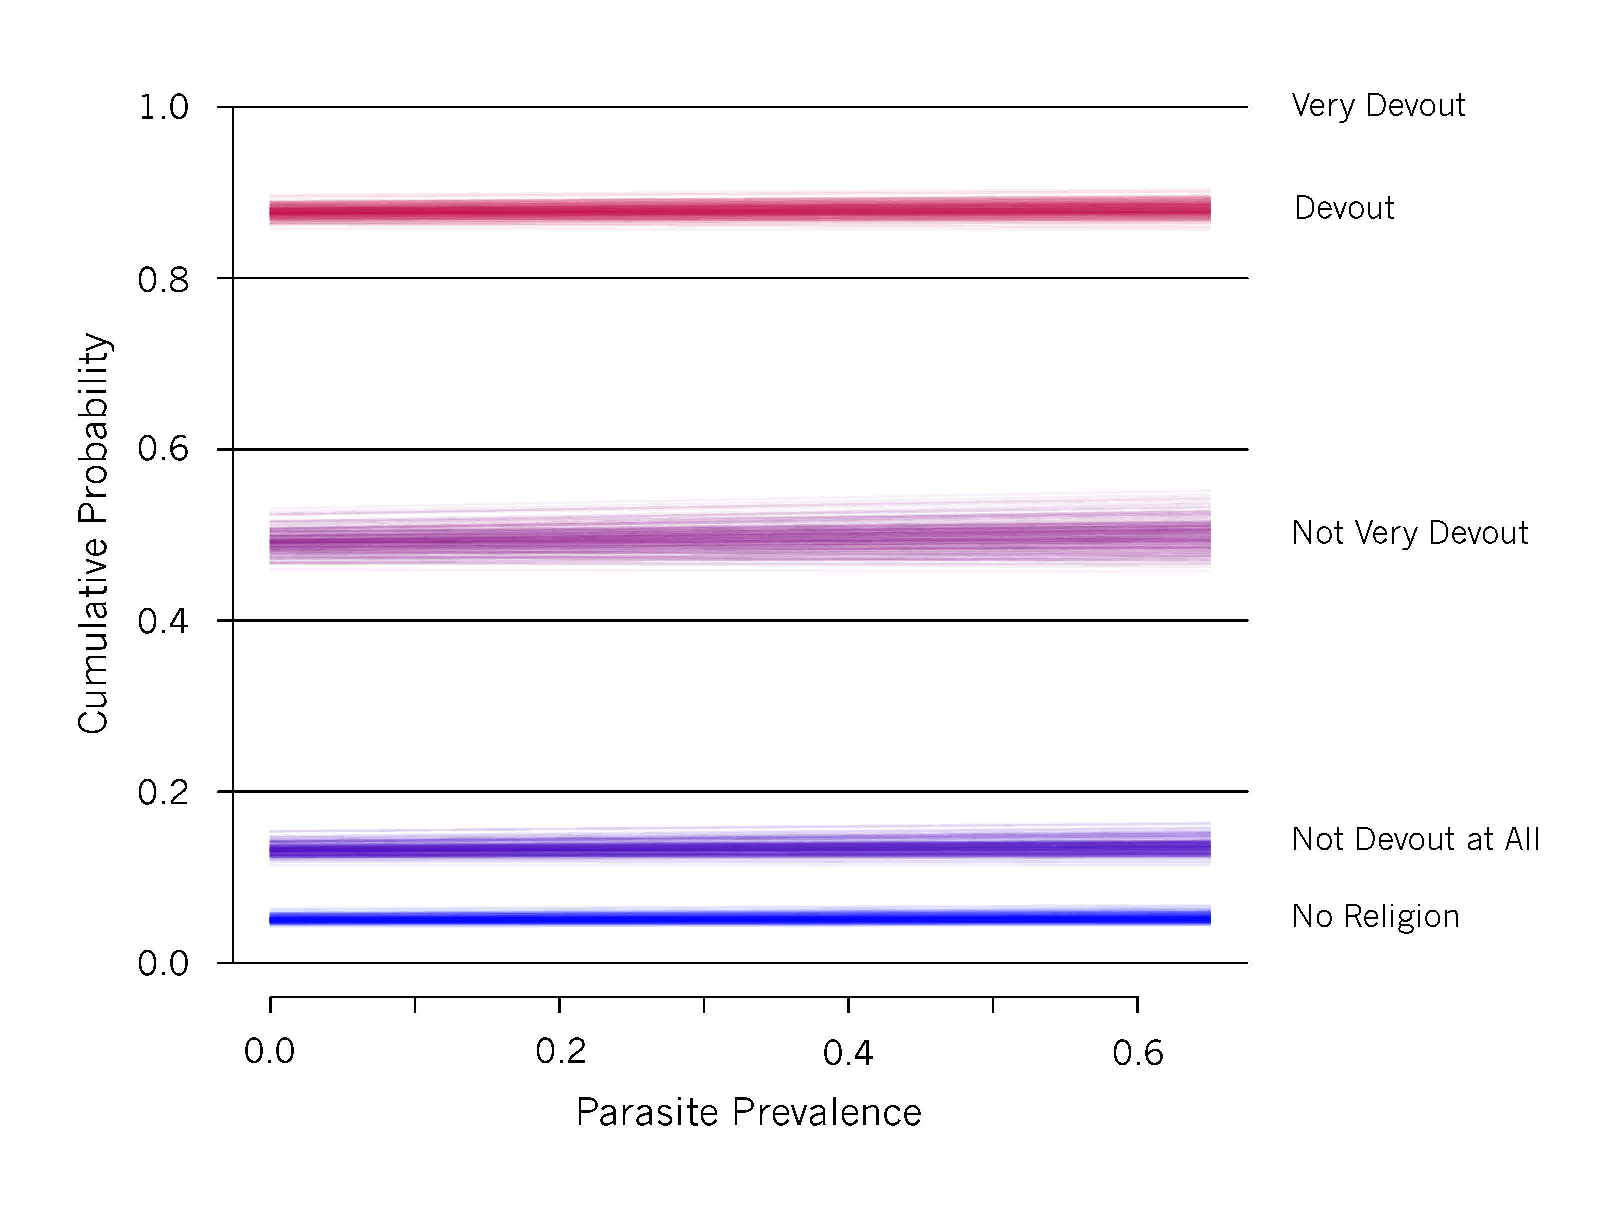
\includegraphics[width=3in]{Figures/WhiteReligiosityModel(WhitenessEquals0)}
        \label{ALubWhitenessAndReligModel:first_sub}
    }     \subfigure[Frame (b) plots the model posterior when a district has a population that is all white. ]
    {
        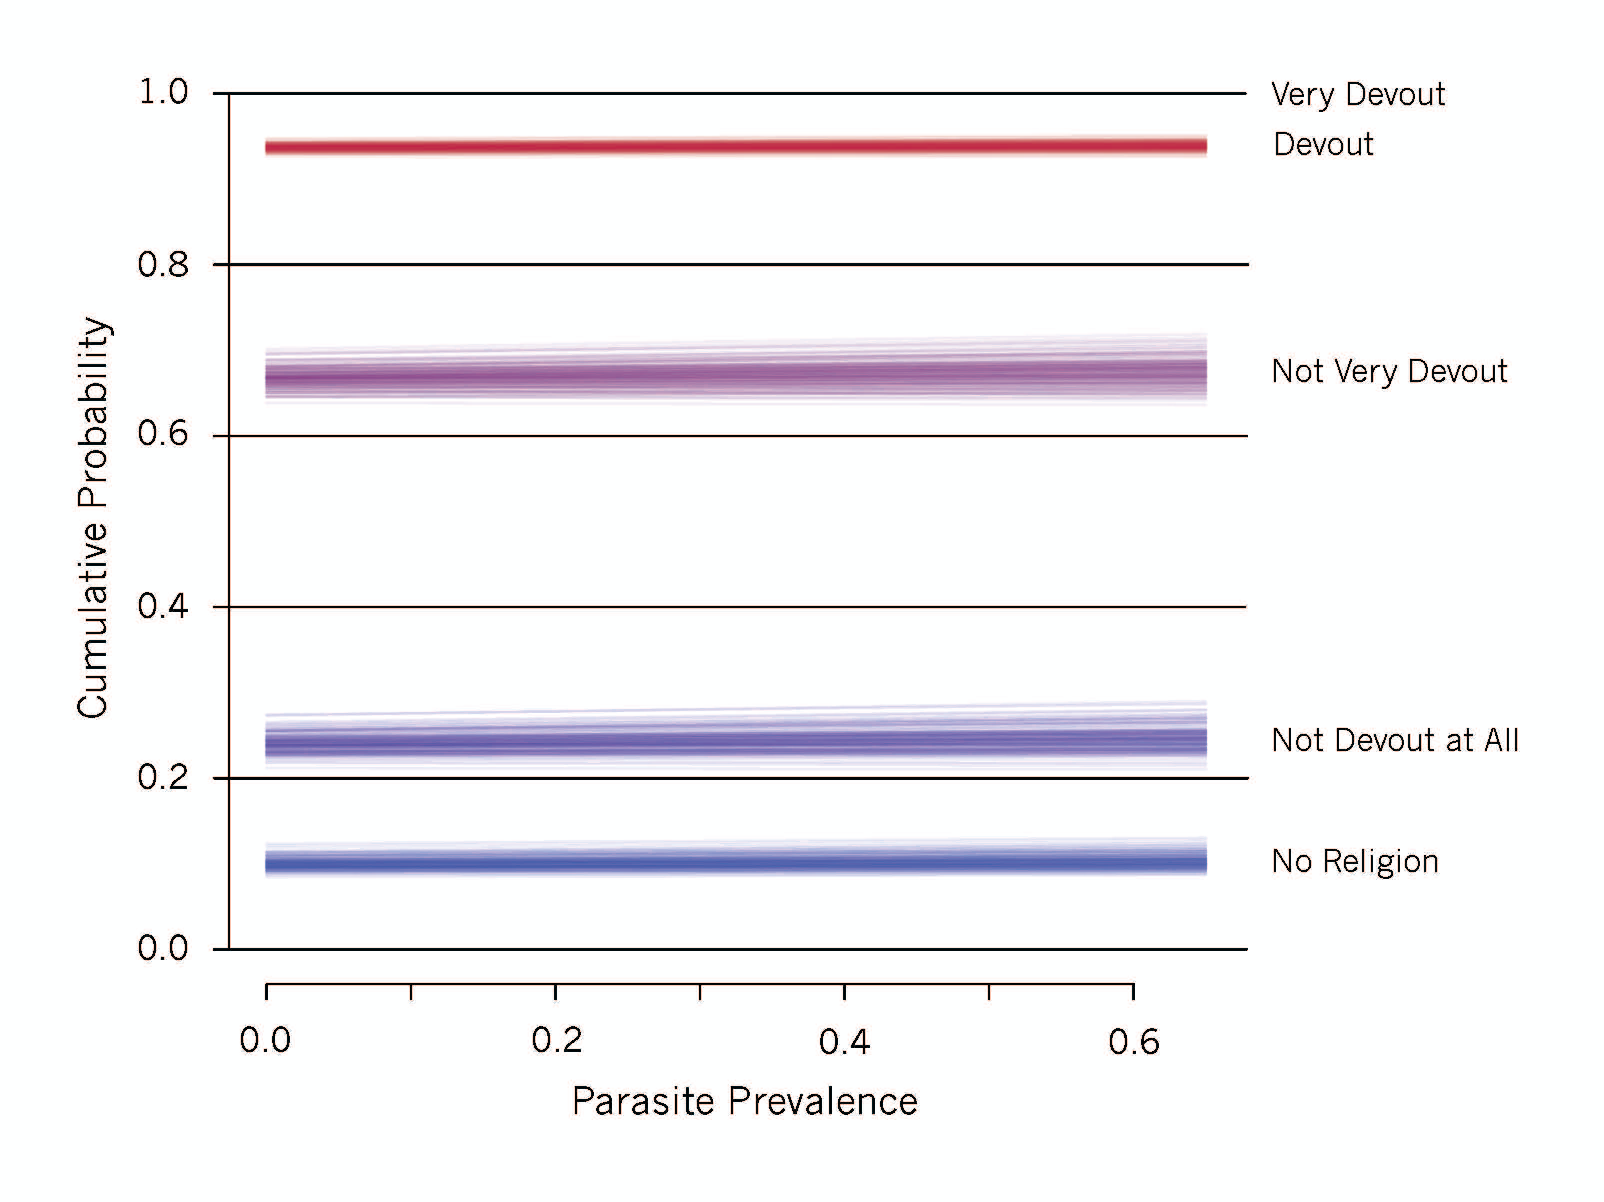
\includegraphics[width=3in]{Figures/WhiteReligiosityModel(WhitenessEquals1)}
        \label{ALubWhitenessAndReligModel:second_sub}
    }
\end{figure} 
 
\section{Discussion}
\subsection{Empirical Results}

\noindent\textit{Parasites and Political Economy}

	Using individual-level data from several thousand individuals in fifty-one districts in eight Latin American countries, and Bayesian methods that retain information on sample size and outcome variance, we re-examine six results from TFE claiming that parasite prevalence is causally associated with a variety of socio-cultural characteristics.  In two cases (Hypotheses 1 and 2), our results show strong associations contrary to those presented TFE; in two cases (Hypotheses 3 and 5), we find strong evidence of an absence of the associations cited in TFE findings; and, in two cases (Hypotheses 4 and 6), we find a reliable association in the direction posited by TFE, but demonstrate that the link between parasite prevalence and the relevant outcome variables is better explained by factors related to structural racism not considered in their analyses.  
	
	We analyze Hypotheses 7-9 in order to compare the explanatory power of parasite prevalence with an alternative suite of factors related to access to sanitation infrastructure and structural racism.  We find consistent evidence in support of predictions linking lack of sewage and sanitation systems to parasite prevalence and the associated cultural variables. The relative count of whites in a district predicts the existence of sewage and sanitation systems, and sewage and sanitation systems and clean water are arguably the most important causal drivers of parasite prevalence \citep{Jongwook2004}.  Indirect evidence presented in this paper suggests that governments may be allocating state resources toward development in a way prejudicial to districts with large non-white populations, implicating structural racism and class privilege as causal drivers of the linkages TFE associate with parasites. TFE's findings arise from mistaking ethnicity and institutionalized racial or ethnic discrimination for parasite load, in a world where colonialism and neo-colonialism generate a correlation between parasites, health outcomes, and ethnicity \citep{better2008institutional, anderson2000gender}.	\\

\noindent\textit{Preference for Democracy}

Contrary to \citet{Thornhill2009}, we find strong evidence that at the district level parasite prevalence is positively and reliably associated with preferences for democracy. This result makes sense, especially in the Latin American context. The populations most likely to be affected by parasitic infection are typically disempowered populations (e.g. afro-descendants and indigenous) who generally have little structural power in government despite having relatively large population sizes in many districts, and would benefit from inclusion in a more democratic governance system. Although our model illustrates that parasite prevalence is positively associated with preferences for democracy, we do not infer direct causality. Parasitic infection does not necessarily cause democratic preference \textit{per se}; the prevalence of parasitic infection simply covaries with many ecological and economic factors that predispose individuals to adopt preferences for democracy. We do note, however, that in populations with high parasite loads, there is a slightly more prevalent belief that neither a democratic nor authoritarian governance system will improve their quality of life\textemdash perhaps a reasonable belief given their experiences. 
	
	Our results show that it is anthropologically ill-informed, at best, to suggest that parasite affected populations value ``autocratic,'' ``xenophobic,'' and ``ethnocentric,'' social organization systems, as suggested by \citet{Thornhill2009}. Rather, we find that parasite affected populations, at least across South America, have higher preferences for democracy than non-affected populations when finely-resolved, non-constructed data are analyzed with appropriate statistical tools.\\
	
	
\noindent\textit{Preference for Individualism}

	Likewise, we find that parasite prevalence is associated positively and reliably with preferences for free-market individualism as opposed to collectivism. However, it is important to note that in absolute terms very few individuals align themselves with free-market policies.  Only 330 of 5,172, or about six percent, of individuals indicated preferences of $>$7 on the 1-10 survey scale, where 10 represented total support of the free market solving problems.  Instead, our findings are driven primarily  by individuals in low parasite regions selecting category 1 (full support of the state solving problems) at higher rates and individuals in high parasite regions selecting intermediate categories higher rates.  It is possible that this effect is driven by two factors: 1) since level of education is positively related to liberal attitudes and increased collectivism \citep{schoon2010social}, and individuals in low parasite (white) regions tend to have higher education status (discussion above), it is likely that education and not parasite prevalence drives attitudes on collectivism. And, 2) individuals in rural areas tend to have more conservative (individualistic) attitudes \citep{fennelly2008rural,ellison2011religion}, and tend to reside in areas with less development (e.g. less sewers/sanitation services). However, the literature on the drivers of individualism/collectivism is vast \citep{triandis2001individualism}, and there are many other possibilities not reviewed here.   \\

\noindent\textit{Gender Equality}

	Contrary to the findings of \citet{Thornhill2009}, we find no evidence that gender equality is negatively associated with parasite prevalence; in fact, we find evidence that the association tends slightly in the opposite direction. \\[12pt] 
 
\noindent\textit{Education/Intelligence}

	While we find evidence that there is a negative association between parasite prevalence and achieved education, parallel to the IQ results of \citet{Eppig2010}, we also find that achieved education is positively associated with district-level racial or ethnic composition (proportion of population that is white) and with access to sewage and sanitation systems.  Districts with greater numbers of non-white citizens have fewer educational opportunities above the lower grades.  They also have less sanitary infrastructure and greater parasite prevalence, but the latter is not required logically or statistically to account for limited educational attainment.  The negative association found by TFE between parasite prevalence and IQ/intelligence (should it exist at all) may be a result of lowered funding for both health and education programs in districts with a low proportion of the dominant ethnic group (`whites' in Latin America).


	We do not dispute the claim that infectious disease can \textit{contribute causally} to the lack of educational attainment, or to the stunting of physical \citep{stephenson1989treatment} or intellectual growth \citep{oknes1994does}.  It has been shown, for example, that parasites affect micro-nutrient absorption and that bioavailability of micro-nutrients, like zinc, affects performance in schools \citep{demment2003providing, neumann2003animal}. Rather, we argue that structural racism and differential access to education are higher-level causal drivers of educational attainment and intellectual development; increased parasite prevalence is only one of the many ways in which structural racism mediates and attenuates the educational achievement of non-whites.  Our findings echo those of \citet{oknes1994does}, who conducted a semi-comprehensive review of studies that evaluated the effects of helmith infection on cognitive performance, and found social and hygenic factors to be more important predictors of cognitive abilities than helmith infections \textit{per se}.\\

\noindent\textit{Violent Crime}

		Contrary to \citet{Thornhill2011}, who argue that parasite prevalence is one of the most ``empircally verified'' variables accounting for violent crime rates, we find no evidence that parasite prevalence is positively associated with violent crime in our Latin American sample. Again, this is not surprising; there are several more plausible drivers of violence in Latin America, such as corruption and bias in police and government, gang conflicts, narco-trafficking operations, racism, and severe wealth inequality.  Parasite prevalence, however, does not appear to cause (or even be associated with) rates of violence. Our results echo those of \citet{hackman2013fast}, who also show that parasite prevalence has no effect on homicide rate when data are analyzed with appropriate statistical tools.   \\
	
\noindent\textit{Religiosity}

	As predicted by \citet{Fincher2012}, we find that parasite prevalence is positively associated with religiosity. However, as cited in \citet{Fincher2012}, there is well established theory linking hardship and religiosity.  Individuals suffering from hardship, including health problems, tend to adopt religious practice as a coping mechanism \citep{koenig2001religion}.  Our results indicate that when controlling for the proportion of population that is white (as an imperfect proxy for suffering and hardship), there is no relationship between parasite prevalence and religiosity.  Furthermore, in Latin America, medical access for impoverished, `non-white' areas often comes via missionary work. The relationship between parasite load and religiosity may thus be explainable at the proximate level, as the result of the association of medical aid with religious organizations, and with the use of religion as a coping mechanism.
	
	

\subsection{Rethinking the Evidence}
\subsubsection{The Construction of Data}
	A serious concern with the methodology employed in the TFE papers is the construction of data. We cite an example from \citet[Electronic Supplement 1.D.]{Fincher2012}:
\begin{quote}
\small
The questions in the World Values Survey (www.worldvaluesurvey.org) comprising Religious Participation and Value 1) were ``How often do you attend religious services?'' We used the proportion of respondents that reported at least once a week. 2) ``How important is God in your life?'' Respondents indicated on a scale from 1 to 10 with 10 being the most important. We used the proportion of those that responded with a 10. And 3) ``How important in religion in your life?'' We used the proportion of those that
indicated religion was very important. All proportions were arcsine square root transformed, standardized, and then summed to be Religious Participation and Value (Cronbach's $\alpha = .94$, $n = 93$).
\end{quote}

 \citet{Fincher2012} begin their analysis with high-quality data compiled from more than 344,000 individual-level surveys. They then discard a vast amount of information by reducing this individual-level data into proportions across 93 countries. Potentially critical information is lost when individual-level records are collapsed to country-level proportions. Further, TFE fail to propagate uncertainty both in the structure of variation across individuals within a country, as well as the uncertainty introduced by sample size variation across countries, rendering all downstream tests of significance unreliable.  Proportions in countries with smaller sample sizes have more uncertainty than proportions from countries with larger sample sizes; however, the regression model has no access to this lost information and the countries with the smallest amount of data have disproportionately high weight in parameter estimation \citep{McDonald2009}. Additionally, outcome variables were constructed by summing several indicators together. This last step is especially perplexing.  It is not clear what empirical reality corresponds to the sum of the standardized arcsine-square-root transformations of the country-level proportions of the individual-level responses of multiple ordered categorical questions.  

	Data construction like that evident in TFE is rarely justified, but when needed should be accompanied by full reporting, at minimum detailing a full explanation as to why the analyst has chosen to \textit{make} composite data in the first place.  Is there a specific theoretical rationale for constructing data instead of using the empirical observations themselves?  Especially important, were any statistical tests performed \citep[see][]{palmer1999detecting}, other than those reported?  The choices entailed in data construction raise concerns over what \citet{Gelman2013} calls `researcher degrees of freedom,' or the possibility that selectively using, transforming, and summing data in various ways can result in spurious correlations with `significant' p-values.  We argue that predictions should be derived from theory in such a way that they can be tested using raw, individual-level, observed data or survey responses.  If there is a pressing reason why it is necessary to combine more than one response into an outcome (e.g., several questions are needed to estimate a latent trait, or multiple observations are needed account for measurement error), then latent trait analysis or measurement error models should be used. 

\subsubsection{Ecological Inference and the Averaging of Data}
Given that TFE make predictions at the individual level\textemdash their hypotheses concern the evolution of human behavior, after all\textemdash the use of state-level or country-level data to test predictions is inappropriate, especially since individual-level data are available.  It is a logical fallacy to infer properties about the nature of individuals who are clustered into groups, from the average properties of the clusters in which individuals are organized \citep{Freedman1999}; Simpson's paradox is an example \citep{yule1903notes, simpson1951interpretation, wagner1982simpson}. When data are pooled into groups, there can be an observed positive trend across groups, even when the trend within every group is negative. Simpson's paradox can be a problem even when individual-level data are used in statistical models where group structure is not modeled appropriately; it is a larger problem when group averages are used in place of individual-level data and modeling of group specific parameters is not possible.
	
	It is necessary to include parasite prevalence as an ecological variable in most models, since parasite prevalence is not a feature of an individual, but of the immediate environment.  Ideally, however, parasite prevalence should be estimated (with error propagation) as near to the local level as possible; our use of district-level analyses is a reluctant compromise in this respect, which should be improved upon by future empirical work.
	

\subsection{Rethinking the Theory}
\subsubsection{Correlation and Causation}
\begin{quote}
\small
In the parasite model of democratization, as parasite stress declines within a region, there is a concomitant evocation, spread, adoption and legalization of liberalized attitudes and values embracing traditionally disenfranchised groups. Consequently, wealth equality, social welfare, economic and educational opportunities, health care, safe public water, sanitation, and rights of holding private property also become widespread \citep[pg117]{Thornhill2009}.
\end{quote}  

This quotation illustrates both the expansive reach of parasites in the TFE literature and some of our reasons for skepticism.  For instance, the use of ``consequently'' betrays a commitment to a causal direction we find less plausible than the reverse.  Following the director general of the World Health Organization, we believe it more plausible  that clean water, sanitation, medication, and health care cause the prevalence of parasites in a region to decline, than \textit{vice versa} \citep{Jongwook2004}.
 
 	While TFE make it clear that they are presenting causal theory based on the interaction of evolutionary psychological mechanisms and environment, they attempt to substantiate their theoretical claims empirically through correlational analysis at the ecological level.  However, the theoretical and causal validity of their arguments cannot be confirmed by ecological-level empirical associations measured by correlation, especially when other more proximate causes like racially-biased access to sanitary infrastructure or clean water would produce the same correlation structures.
 	
\subsubsection{Evolved Psychological Mechanisms and Human Sociality}
Across most of the TFE literature, parasite prevalence is thought to affect downstream cultural characteristics primarily through evolved psychological mechanisms that modulate sociality and in-group/out-group biases; for example, \citet{Fincher2012} argue broadly that key features of hominin sociality have been shaped by parasitic disease through selection for ``ancestrally adaptive feelings, attitudes, and values about and behaviors toward out-group and in-group members,'' due to the increased likelihood of infection and severity of infections acquired via interaction with outsiders \citep[pg60]{Fincher2012}. 

While it is clear that parasitic diseases have constituted a serious source of morbidity and mortality in human evolutionary history, we remain cautious of arguments about the evolutionary dynamics of complex systems when such dynamics are not modeled formally. There is no \textit{a priori} reason to believe that natural selection should act to produce psychological mechanisms that minimize morbidity or mortality from disease, as it more closely approximates a process which maximizes the geometric mean of fitness \citep{Gillespie1977,Boyce1987}, rather than one which minimizes the probability of mortality \citep[see][on senescence]{kirkwood1991evolution, williams2001pleiotropy}. The net fitness consequences of interaction with out-group members requires cost-benefit analysis covering the increased probability of parasite exposure and the severity of associated consequences, as well as the benefits that might follow from the interaction with out-group members.  There is no \textit{a priori} basis for believing the costs to outweigh the benefits.  Under a formalized model, one could estimate the contexts (ratios of the costs imposed by the increase in parasite stress due to interactions with out-group members, relative to the benefits of interactions with out-group members) in which the parasite-stress theory of sociality might apply. Without such formal models, it is impossible to critically evaluate the parasite-stress theory of sociality. 

	We do not dispute the claim that humans could have evolved culturally or biologically encoded behavioral mechanisms that utilize information on local parasite prevalence to adaptively alter behavioral responses\textemdash in fact, we agree that there is fairly strong evidence of species-general adaptive behavioral responses to contexts in which disease transmission is likely \citep{curtis2001dirt,curtis2011disgust}, as well as adaptive culture-specific taboos \citep[eg. prohibitions on eating pork,][]{diener1978ecology}, that function to minimize exposure to pathogens in specific contexts. We would argue, however, that adaptations concerning sociality in humans will be complex, context dependent, and tightly constrained by local costs \textit{and} benefits. 
	
	 There are numerous examples where humans behave in ways that increase the exposure to pathogens [eg. prostitution and high risk sexual activity \citep{Carcamo2012765}, body modification \citep{tweeten1998infectious}, settlement in densely populated cities \citep{de1995does}, trade/travel \citep{ali2006global}, medical work \citep{pearson1992nosocomial}, farming \citep{matthys2006urban}, and the rearing of domesticated animals \citep{vaughn1992epidemiology}].  There are, however, principled reasons why all of these behaviors may be adaptive (or may be produced by psychological mechanisms designed to produce adaptive behavior) in specific ecological contexts, despite fact that they all increase the risk of disease transmission. 
	 
	 Medical work, for example, increases one risk of disease morbidity and mortality \citep{pearson1992nosocomial}, but it also augments one's prestige and social class, increases power in the mating market, and carries significant financial rewards, which are translatable into security for one's offspring. Likewise, the domestication of dogs, pigs, poultry, horses, and cattle has led to an increase in the prevalence of many serious diseases, including rabies \citep{wandeler1993ecology},  chlamydiosis \citep{jacob2005avian}, avian influenza \citep{mounts1999case}, eastern equine encephalitis \citep{jacob2005avian}, and trichinosis \citep{gould1970trichinosis}. However, dogs and horses have been important in transportation, hunting, and protection \citep{brown2012ancient,koster2008hunting}, and cattle and other livestock transform inedible roughage into edible meat, blood, and milk, which allow for residence on otherwise marginal land  \citep{mace1993transitions}. 
	
	 Appreciated in socio-ecological context, the ethnographic and epidemiological literatures provide a wide range of case studies in which behavioral responses function to increase the risk of disease/parasite transmission \citep{molineaux1980garki, vaughn1992epidemiology, allen2008mice,  rothenberg2009hiv, parad2012psychological, pittphilsci9767}, because they also increase reproduction, material wealth, or otherwise augment fitness considerations. Given that many human-parasite/disease systems seem to be causally driven by what seems to be locally adaptive human behavior, we remain skeptical of verbal models claiming that human sociality has been evolutionarily designed to universally minimize the risk of parasite/disease transmission.
 
\subsection{Conclusions and Future Directions}
		Behavioral responses to disease environments are matters of the immediate socio-ecological context, and evolutionary analysis gains power as it approaches this scale \citep{winterhalder1997evolutionary}.  Ecological regression on metrics aggregated into single values at the country or state level occludes the fine-scale dynamics of human parasite systems, and risks capturing spurious correlations created by averaging data at national levels [Simpson's paradox \citep{simpson1951interpretation} and the ecological inference fallacy \citep{Freedman1999}], the discarding of variance information \citep{draper1995assessment}, the file drawer effect \citep{cassey2004survey, palmer1999detecting}, and data exclusion \citep{palmer1999detecting} or construction. Cost-benefit analysis linking parasite prevalence and human behavioral and cultural consequences requires modeling the dynamics of human parasite systems at the appropriate level, using locally-resolved data on parasite prevalence, and individual-level data on behavior, cultural beliefs, and psychological measures. 

	Parasites may well prove to be a factor in human social evolution, but we do not have a sound scientific basis for affirming that they are.  There are two bases for the reservations we express here:  1) Recent developments in evolutionary anthropology \citep{smith2001tree, laland2011sense} point us toward a much broader set of approaches and requirements that must be addressed in making the theoretical case; and, 2) there are serious analytical flaws in the TFE analyses which, when corrected with more appropriate methods and data, lead us  \citep[and][]{hackman2013fast} to  reliable results that strongly diverge from theirs.

%%%%%%%%%%%%%%%%%%%%%%%%%%%%%%%%%%%%%%%%%%%%%%%%%%%%%%%%%%%%%%%%%%%%%%%%%%%%%%%%%
% BIBLIOGRAPHY
\bibliographystyle{spbasic}
\bibliography{AJHB-LatexPaper}



%%%%%%%%%%%%%%%%%%%%%%%%%%%%%%%%%%%%%%%%%%%%%%%%%%%%%%%%%%%%%%%%%%%%%%%%%%%%
\end{document}

